\chapter{Materiales y métodos}
\thispagestyle{empty}

\section{Materiales}

Dada la exigencia de grandes volúmenes de datos en los modelos de aprendizaje profundo, optaremos por la utilización de un conjunto de datos sintéticos. Para ello, se simularán imágenes fotorrealistas a partir de la selección de diversos modelos 3D, que abarcan desde modelos faciales hasta modelos de cuerpo entero. Además, se implementará un \textit{pipeline} específico para garantizar que todos los modelos se encuentren de forma estandarizada.

\subsection{Modelos 3D}
Tras una análisis exhaustivo de las bases de datos disponibles de modelos 3D de personas, se optó por la combinación de múltiples conjuntos de datos públicos. El objetivo fue crear un conjunto de datos unificado que fuera a la vez realista y diverso. Este conjunto final incluye tanto modelos faciales como de cuerpo completo, todos ellos asociados con sus correspondientes texturas.

\subsubsection{Modelos faciales}
Se seleccionaron los siguientes conjuntos de datos: HeadSpace \cite{60}, H3DS-net \cite{61}, Stirling ESRC 3D Face \footnote{Stirling ESRC 3D Face disponible en https://pics.stir.ac.uk/ESRC/}  y DI4D\_UGR \footnote{Conjunto de datos proporcionado por el tutor.}.

El conjunto de datos de Headspace \cite{60} es un conjunto de imágenes en 3D de la cabeza humana, que consta de 1519 sujetos que llevan gorros de látex ajustados para reducir el efecto de los peinados (Figura \ref{fig17}). Este conjunto presenta múltiples ventajas, entre las cuales destacan su excelente resolución y la inclusión de metadatos útiles que facilitan la selección de un subconjunto de datos adecuado. Sin embargo, debido a que este tipo de modelos pueden introducir sesgos al no representar casos realistas, se utilizará un número limitado de ellos para complementar el conjunto de modelos final.

\begin{figure}[H]
	\centering
	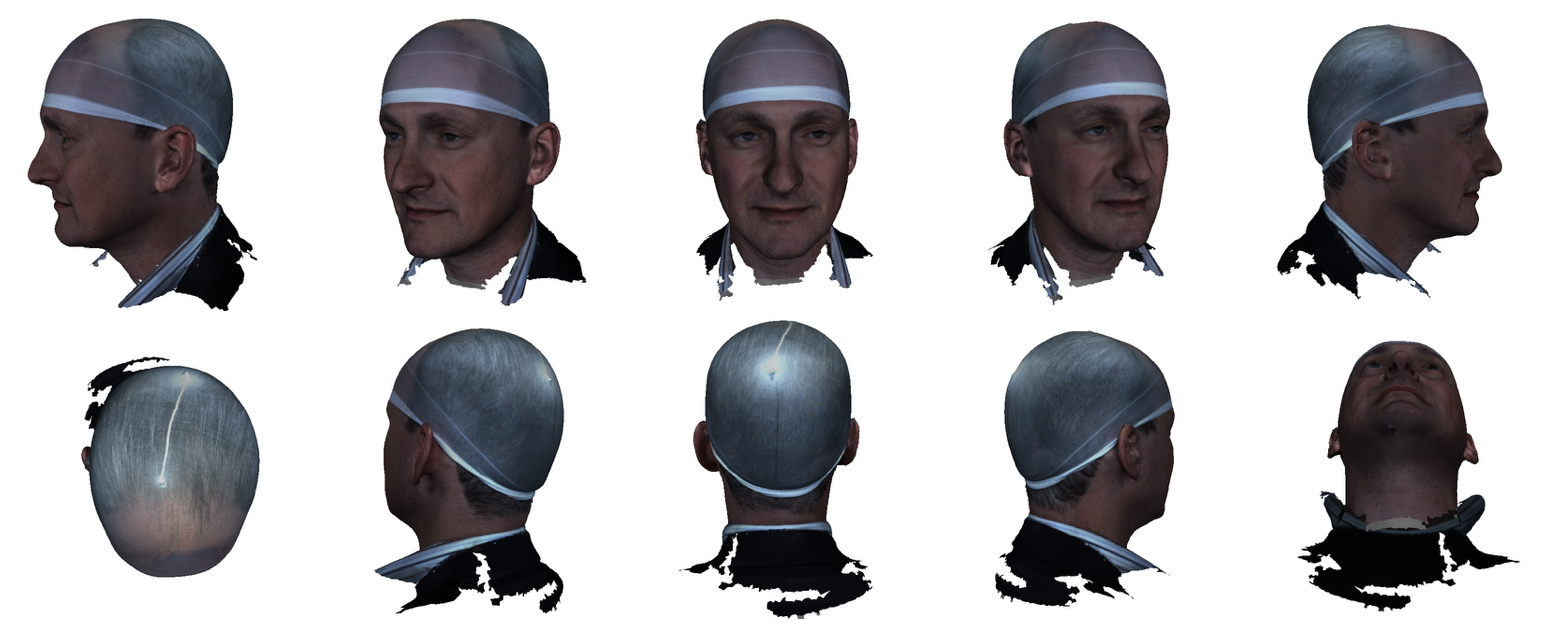
\includegraphics[scale=0.075]{imagenes/cap4/headspace.png}
	\caption[Ejemplos HeadSpace 3D.]{Ejemplos de modelos en HeadSpace 3D.}
	\label{fig17}
\end{figure}

H3DS-net \cite{61} contiene escaneos texturizados en 3D de la cabeza completa con una alta resolución (Figura \ref{fig18}). Este conjunto comprende un total de 23 modelos, todos ellos con los ojos cerrados, lo que proporciona una variabilidad adicional en los datos.

\begin{figure}[H]
	\centering
	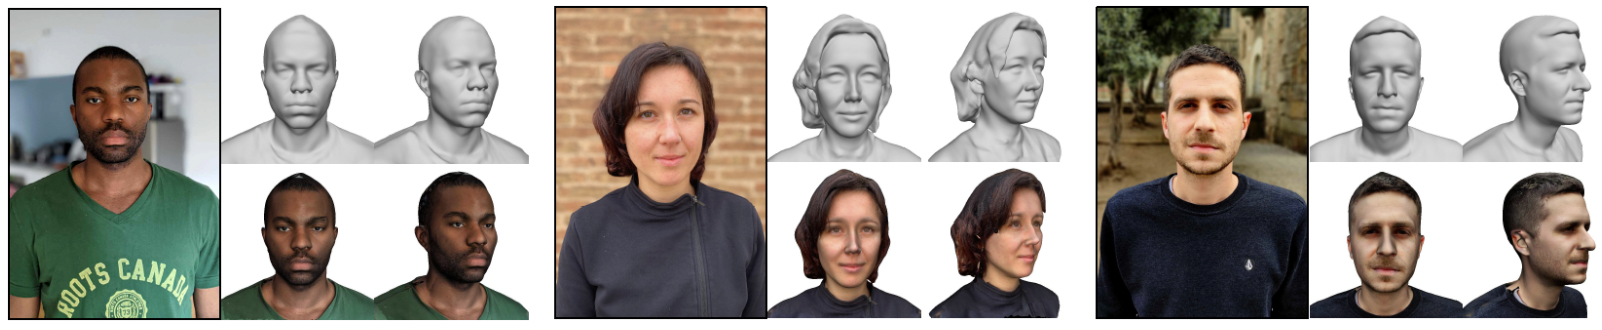
\includegraphics[scale=0.18]{imagenes/cap4/h3dsnet.png}
	\caption[Ejemplos H3DS-net.]{Ejemplos de modelos en H3DS-net.}
	\label{fig18}
\end{figure}

Stirling ESRC 3D Face es una colección que contiene 99 sujetos con redecilla en el pelo (Figura \ref{fig18.1}). Cada uno de ellos contiene múltiples modelos faciales en 3D que capturan una variedad de expresiones faciales.

\begin{figure}[H]
	\centering
	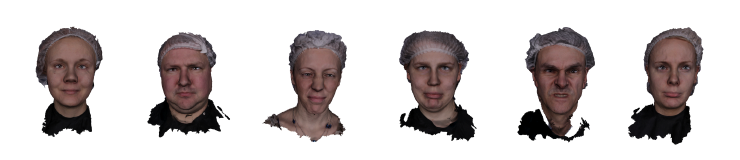
\includegraphics[scale=0.85]{imagenes/cap4/stirling.png}
	\caption[Ejemplos Stirling ESRC 3D Face.]{Ejemplos de modelos en Stirling ESRC 3D Face.}
	\label{fig18.1}
\end{figure}

DI4D\_UGR es un conjunto de datos adquiridos en la Universidad de Granada, concretamente en el laboratorio A!4HumanID Lab del instituto Dasci. Los modelos fueron adquiridos utilizando un dispositivo de gran calidad basado en fotoantropometría, llamado DI4D Pro. El conjunto de datos consta de 40 sujetos, cada uno de los cuales fue escaneado mostrando diferentes expresiones faciales, tales como sonrisa, enfado, tristeza, sorpresa o neutral (Figura \ref{fig18.2}).

\begin{figure}[H]
	\centering
	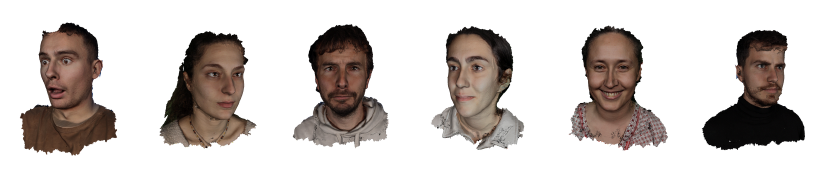
\includegraphics[scale=0.8]{imagenes/cap4/di4d.png}
	\caption[Ejemplos DI4D\_UGR.]{Ejemplos de modelos en DI4D\_UGR.}
	\label{fig18.2}
\end{figure}

Si bien se investigaron otros conjuntos de datos como FaceVerse \cite{64} o CASIA \footnote{CASIA disponible en http://biometrics.idealtest.org/}, estos fueron descartados debido a problemas como la baja calidad, formatos incompatibles y escalas no reales.

\subsubsection{Modelos de cuerpo entero}
Se han seleccionado los siguientes conjuntos de datos: HuMMan \cite{62}, People Snapshot \cite{63} y Render People \footnote{RenderPeople disponible en https://renderpeople.com/es/}.

HuMMan \cite{62} es un conjunto de datos 3D que consta de 153 sujetos humanos, con una amplia cobertura de sexos biológicos, edades, formas del cuerpo y poblaciones (Figura \ref{fig19}). Cada sujeto contiene 2-3 secuencias, y cada secuencia contiene aproximadamente 20 modelos. Este \textit{dataset} destaca por la gran cantidad de poses disponibles para cada modelo.

\begin{figure}[H]
	\centering
	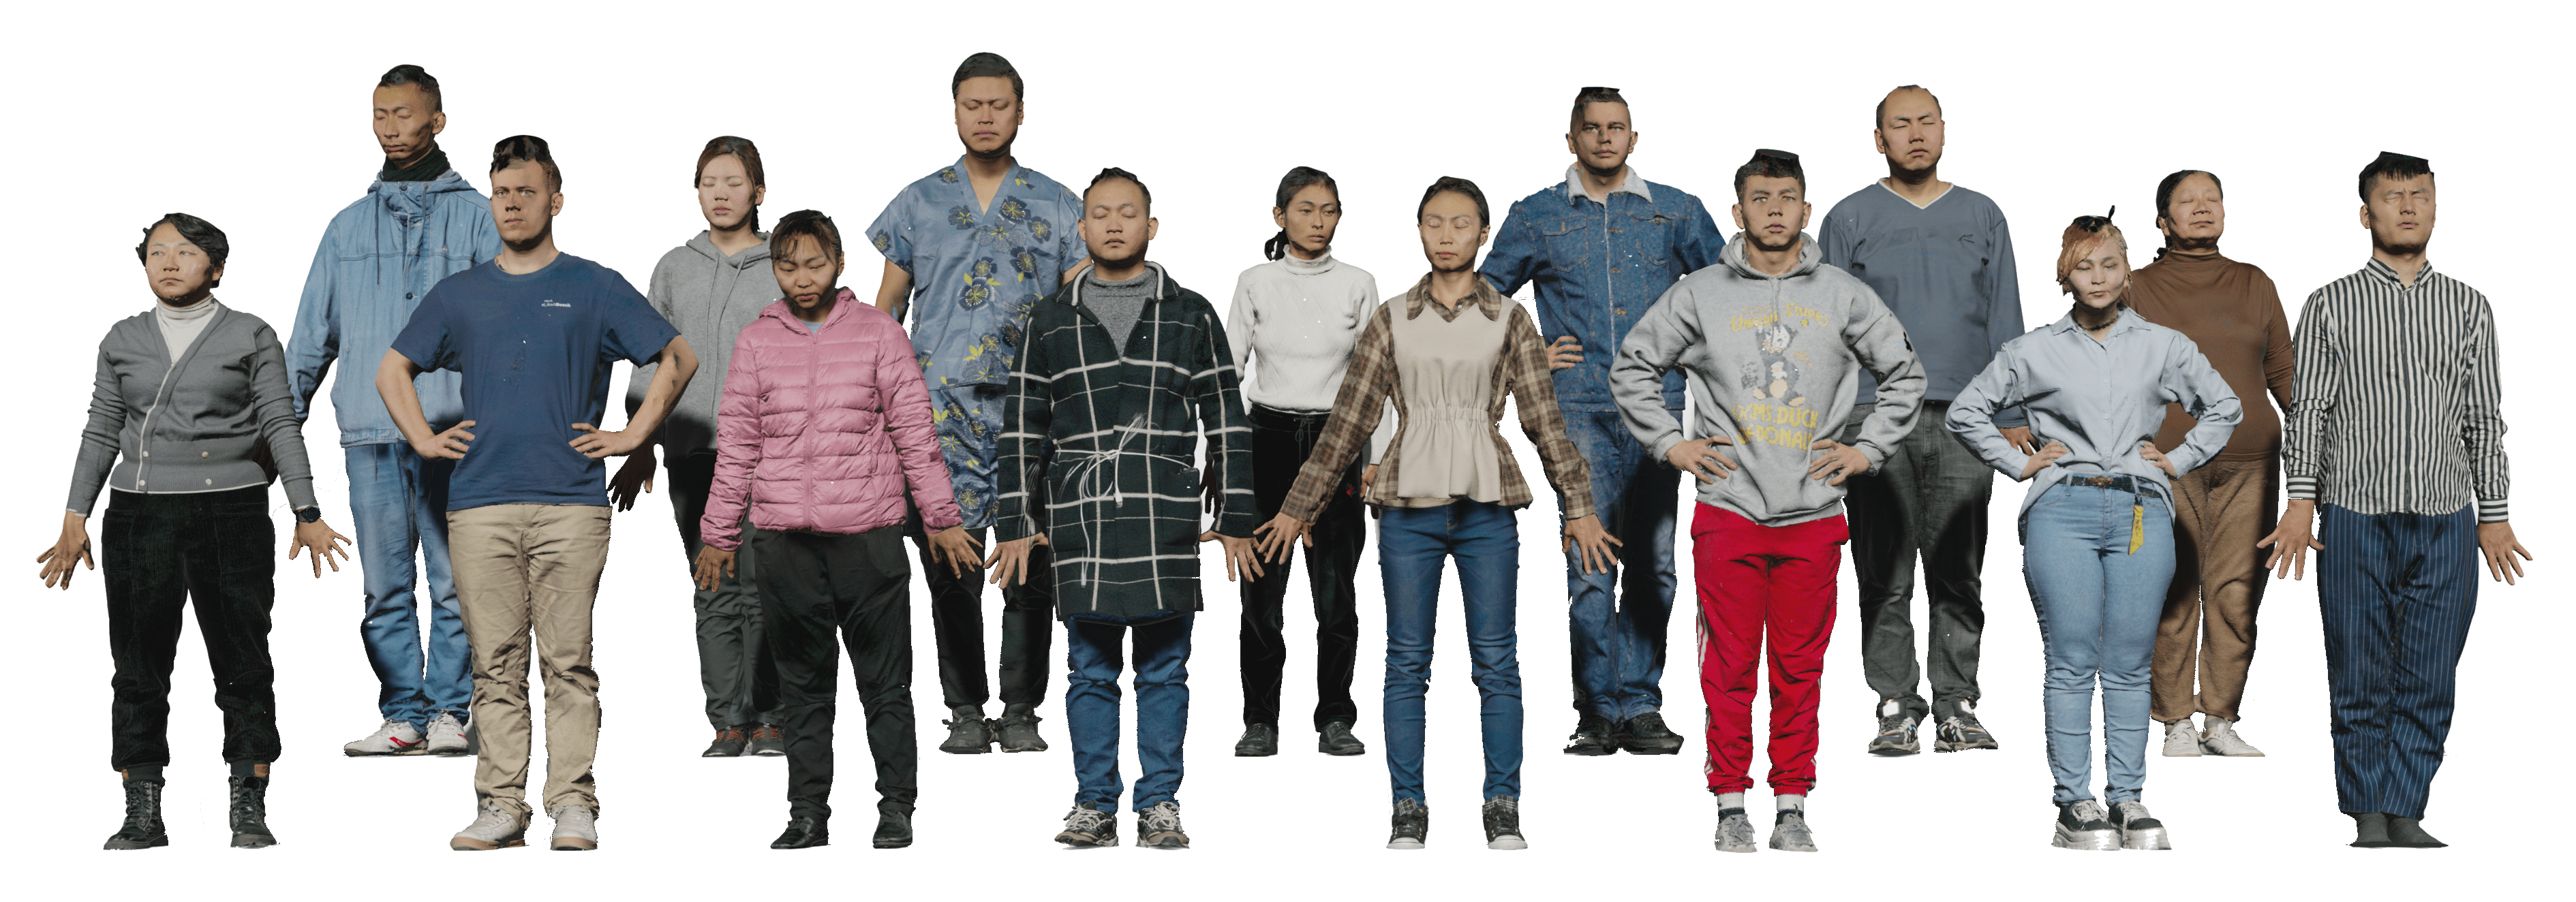
\includegraphics[scale=0.4]{imagenes/cap4/humman.png}
	\caption[Ejemplos HuMMan.]{Ejemplos de modelos en HuMMan.}
	\label{fig19}
\end{figure}

People Snapshot \cite{63} contiene 24 sujetos 3D con textiras adaptadas a diferentes situaciones tales como casual, deporte y actividades al aire libre (Figura \ref{fig20}).

\begin{figure}[H]
	\centering
	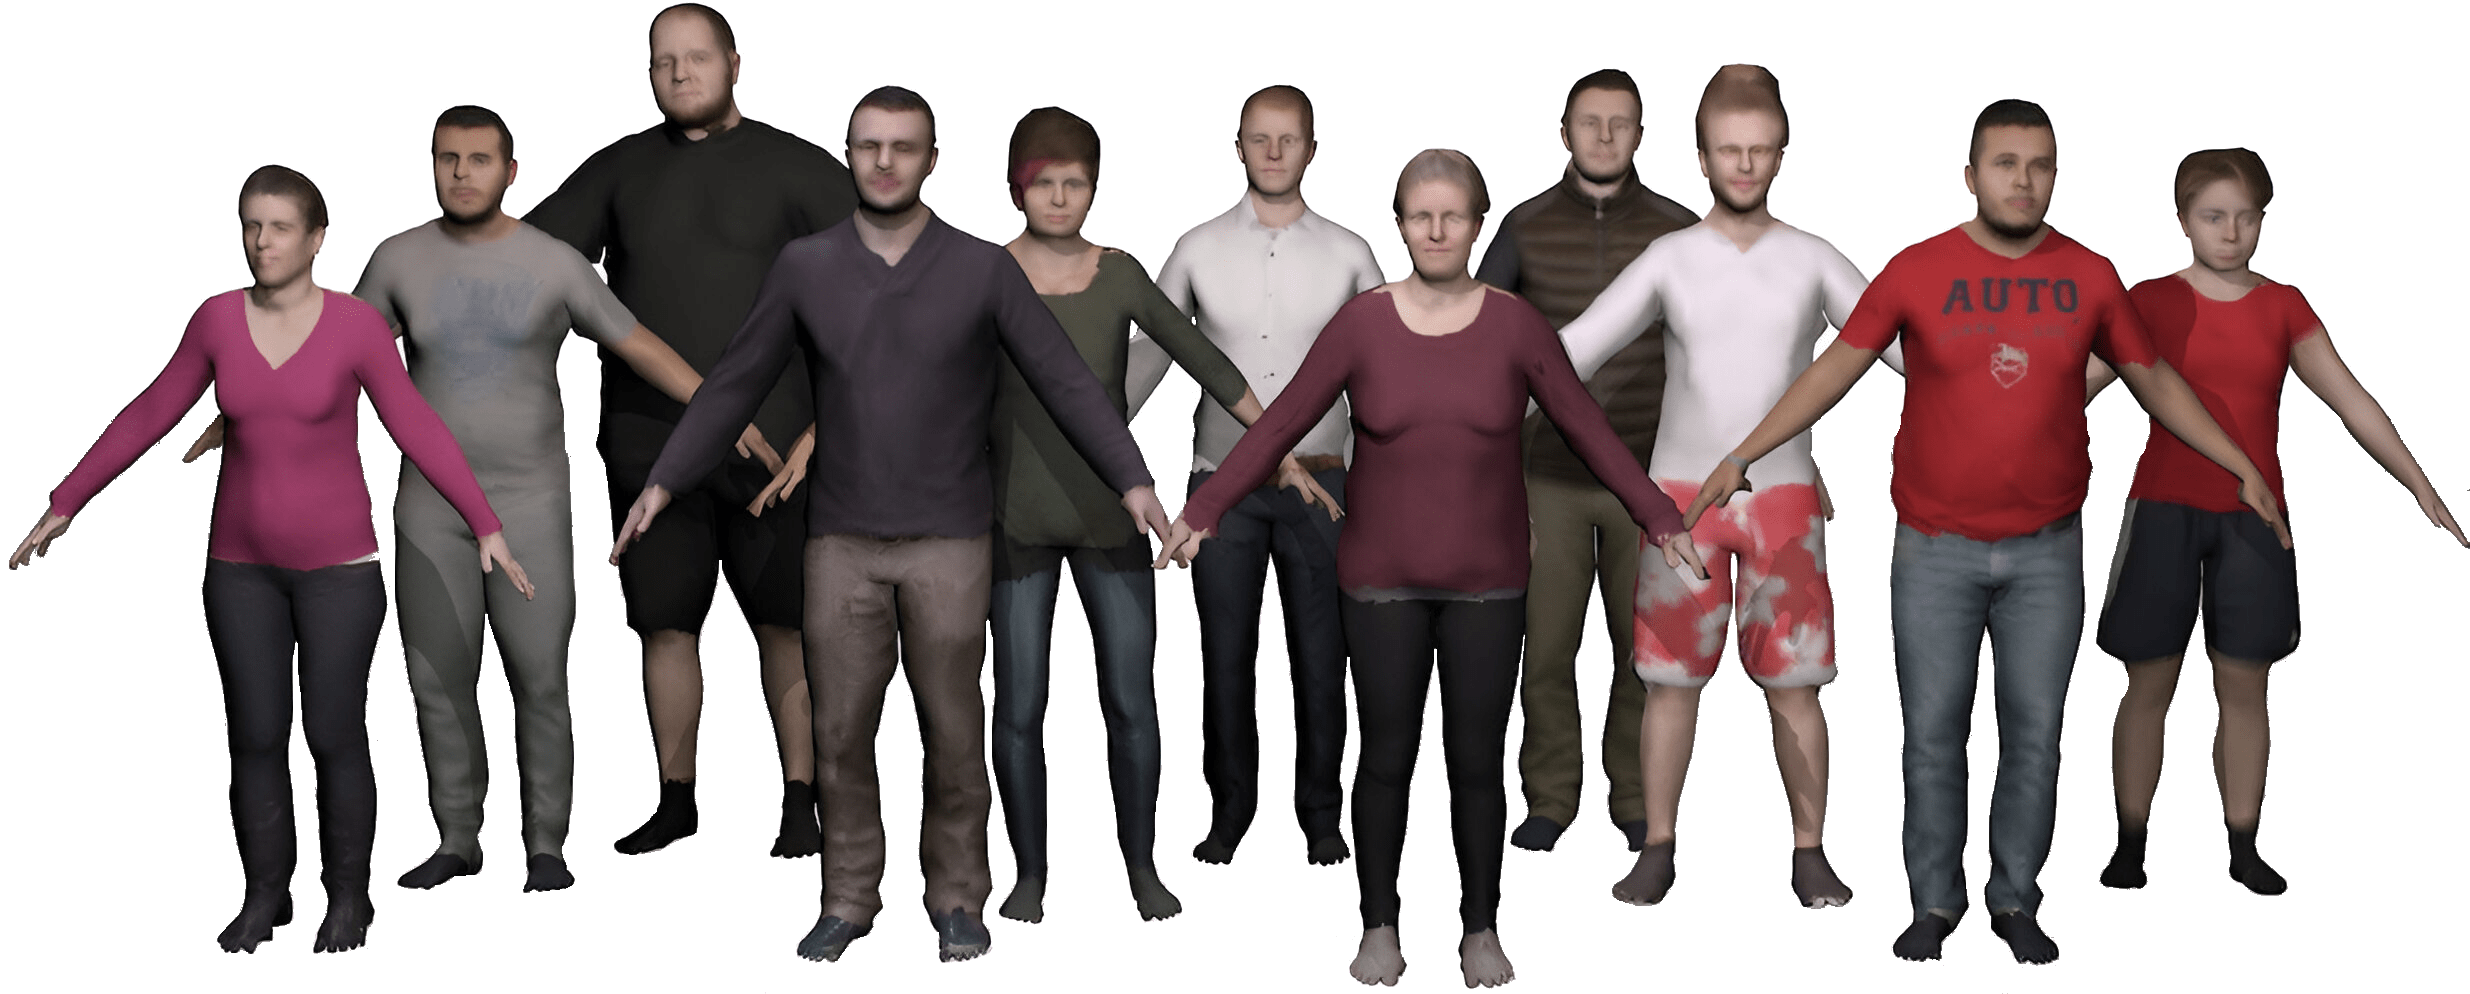
\includegraphics[scale=0.5]{imagenes/cap4/snapshot.png}
	\caption[Ejemplos People Snapshot]{Ejemplos de modelos en People Snapshot.}
	\label{fig20}
\end{figure}

RenderPeople es una empresa privada especializada en la creación de modelos humanos en 3D. Existen modelos disponibles para comprar, pero dado su costo, hemos decidido emplear exclusivamente aquellos gratuitos que están disponibles. Aunque únicamente hay 2, estos son bastante realistas y presentan situaciones que no se contemplan en los anteriores modelos (Figura \ref{fig21}).

\begin{figure}[H]
	\centering
	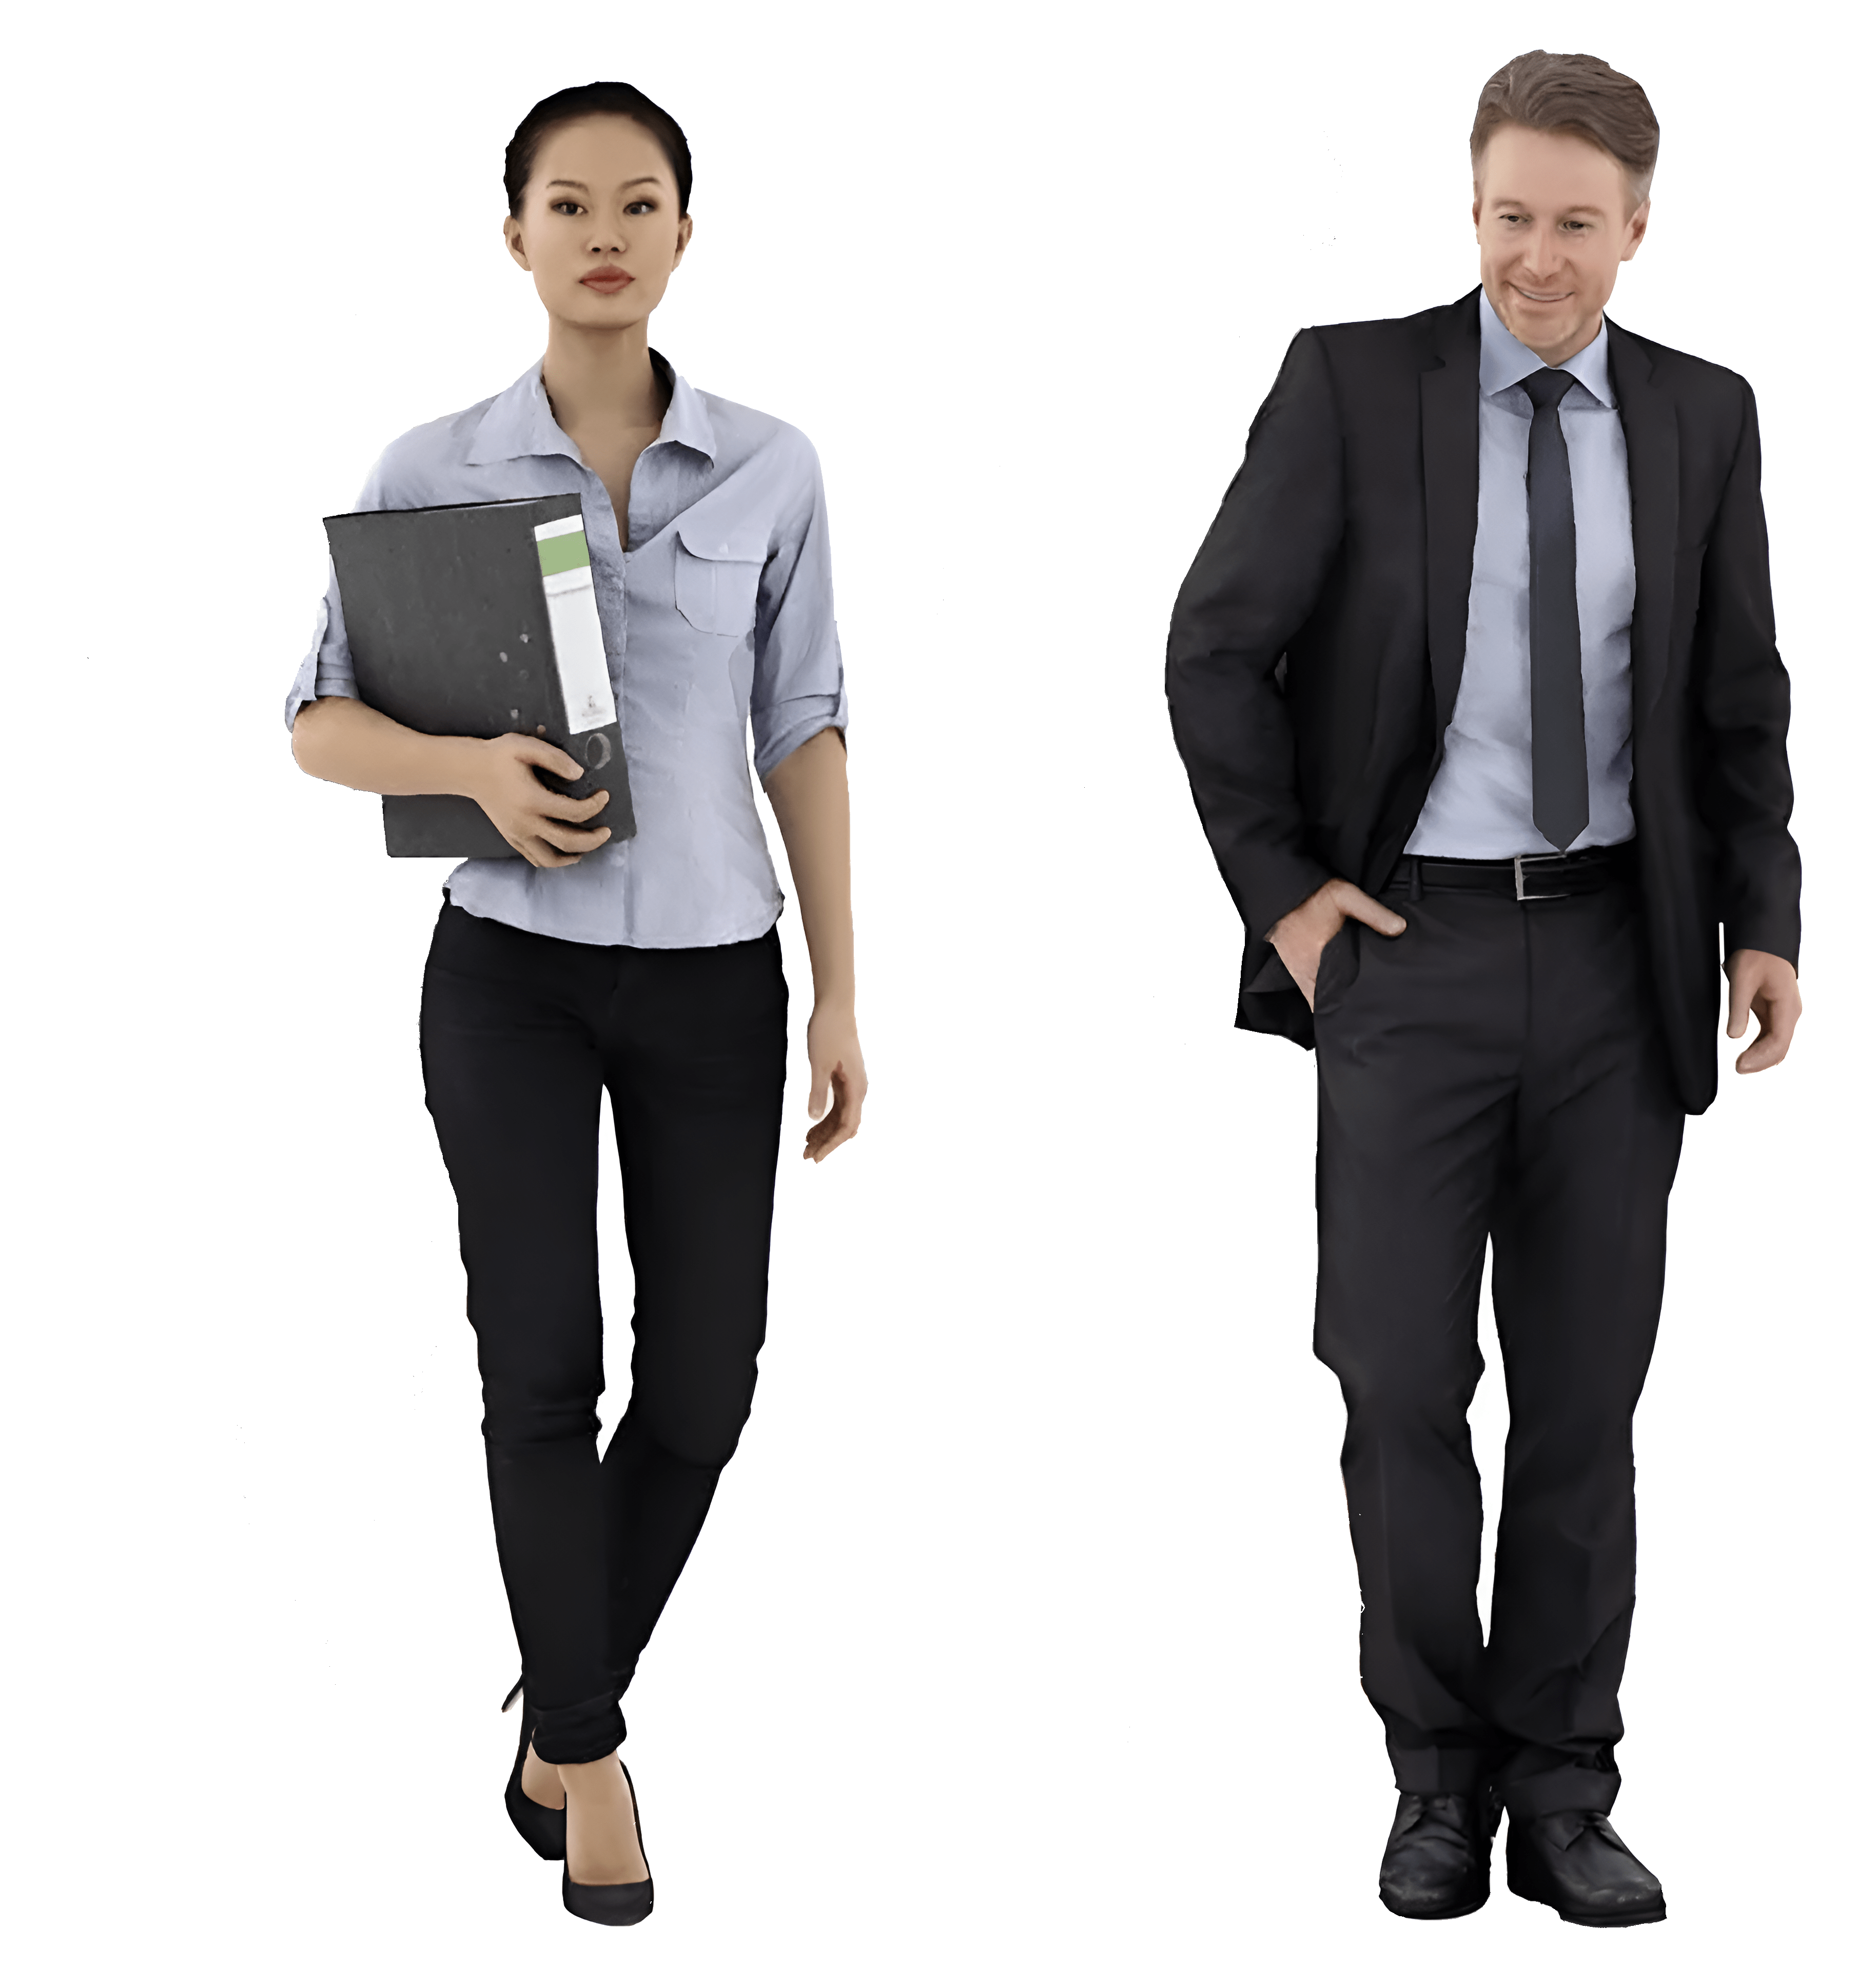
\includegraphics[scale=0.04]{imagenes/cap4/renderpeople.png}
	\caption[Ejemplos Render People]{Ejemplos de modelos en Render People.}
	\label{fig21}
\end{figure}

\subsubsection{Selección del subconjunto de modelos}

Ante la gran cantidad de modelos disponibles, surge la necesidad de elegir un subconjunto de modelos adecuado, combinando modelos faciales y de cuerpo completo.
Inicialmente, se seleccionaron 300 modelos 3D, de los cuales 206 son modelos faciales y 94 son modelos de cuerpo completo.

En cuanto a los modelos faciales, se seleccionaron 23 modelos de H3DS-net, compuestos por 13 masculinos y 10 femeninos, todos de ascendencia europea. De HeadSpace, se seleccionaron 93 modelos, con una distribución de 46 masculinos y 47 femeninos, cubriendo una amplia gama de edades y representando diversas ascendencias, incluyendo europea, asiática, africana o mixta. Se seleccionaron 50 modelos de la base de datos Stirling ESRC 3D Face, con 43 femeninos y 7 masculinos, mayoritariamente de ascendencia europea. Por último, se seleccionaron 40 modelos de DI4D\_UGR, con una distribución de 17 femeninos y 23 masculinos, todos de ascendencia europea.

Por otro lado, en cuanto a los modelos completos, se seleccionaron 2 modelos de RenderPeople, uno masculino y otro femenino, ambos de ascendencia europea. De People Snapshot, se eligieron 24 modelos, siendo 16 masculinos y 8 femeninos, todos de ascendencia europea. Finalmente, se seleccionaron 68 modelos de HuMMan, distribuidos equitativamente en 34 masculinos y 34 femeninos, con una variedad de ascendencias incluyendo asiática, africana y europea.

Estas selecciones se hicieron con el propósito de garantizar una amplia diversidad en términos de sexos biológicos, ascendencias y poses, teniendo en cuenta las bases de datos disponibles. Sin embargo, a pesar de que inicialmente la muestra era de 300 modelos 3D, después de algunas pruebas preliminares, se descartaron 23 modelos debido a su potencial impacto negativo en el aprendizaje, lo que resultó en un conjunto final de 277 modelos.

\subsection{Preparación del conjunto de datos}

\subsubsection{Procesamiento de modelos 3D}

Al contar con un conjunto de datos compuesto por múltiples conjuntos, cada uno con una escala específica, ya sea en centímetros o metros, y dispuestos de manera diversa, surge la necesidad de normalizar la escala y alinear los modelos con respecto a un punto de referencia. Para esto, se empleará el centro de los ojos como punto de origen (0, 0, 0), dado que son fácilmente visualizables, se ubican en una posición central y están presentes tanto en los modelos faciales como en los de cuerpo completo. Este procesamiento se produce para luego poder generar correctamente las imágenes a distintas distancias.

La normalización de la escala se lleva a cabo mediante transformaciones de escala, multiplicando o dividiendo por un factor de 100. Esta se realiza solo en algunos modelos, para que todos estén a la misma escala.

Para alinear los modelos, en primer lugar se aplicó un \textit{script} de \textit{Python} para realizar transformaciones (específicas para cada conjunto de datos) con el objetivo de posicionarlos de frente. Posteriormente, se desarrolló un programa en \textit{Python} que utiliza librerías como \textit{VTK}, \textit{PyVista} y \textit{Trimesh} para la manipulación de mallas 3D, junto con \textit{Mediapipe} para la detección de rostros. El proceso implica tener un modelo de referencia ya alineado manualmente, junto con 13 puntos de referencia faciales 3D (incluyendo la nariz, los ojos y la boca) obtenidos mediante \textit{Mediapipe}. Después, dado un nuevo modelo sin alinear, se calculan sus puntos de referencia correspondientes y se determina y aplica la matriz de transformación entre estos puntos y los del modelo de referencia.

A excepción de algunos ajustes manuales en los modelos de HeadSpace y HuMMan, el proceso se automatizó de forma efectiva.

\subsubsection{Generación de imágenes faciales sintéticas}

Una vez procesados los modelos 3D, se procedió a generar el conjunto de imágenes faciales. Para ello, se utilizó un \textit{script} en \textit{Blender} cuyo pseucódigo está en el Algoritmo \ref{alg:render_images}. 

\begin{algorithm}
	\caption{Generación de imágenes}\label{alg:render_images}
	\begin{algorithmic}[1]
	\State $model\_iters = 14$
	\State $image\_width = 224$
	\State $image\_height = 224$
	\State $distances = [50, 55, 60, ..., 500, 600]$
	\State $focals = [35]$
	\For{\textbf{each} $model$ \textbf{in} $models$}
		\State \Call{load\_model}{$model$}
		\For {\textbf{each} $d$ \textbf{in} $distances$}
			\State \Call{set\_distance}{$d$}
			\For{\textbf{each} $f$ \textbf{in} $focals$}
				\State \Call{set\_focal}{$f$}
				\For{$i = 0$ \textbf{to} $model\_iters-1$}
					\State $background \gets \Call{select\_random\_background}{}() $
					\State \Call{set\_background}{$background$}
					\State $rx \gets \Call{uniform}{-30, 30}$ %\Comment{Degrees}
					\State $rz \gets \Call{uniform}{-70,70}$
					\State \Call{apply\_rotation}{$rx, 0, rz$}
					\State \Call{apply\_random\_translation}{}()
					\State \Call{set\_random\_ilumination}{}()
					\State \Call{save\_image}{}()
				\EndFor
			\EndFor
		\EndFor
	\EndFor
	\end{algorithmic}
\end{algorithm}

A continuación, se detallan las tareas específicas llevadas a cabo para cada modelo del conjunto de datos 3D:

\renewcommand{\theenumii}{\arabic{enumii}}

\begin{enumerate}
	\item Carga el modelo y lo posiciona a una distancia específica de la cámara. Se seleccionaron 35 distancias diferentes, que van desde 50 cm hasta 6 m, con incrementos graduales de 5 cm, 10 cm, 20 cm y 25 cm.
	\item Posteriormente, para cada distancia, se ajusta la distancia focal de la cámara. En este caso, solo se utilizó la focal de 35 mm.
	\item A continuación, para cada distancia focal, se realizan 14 iteraciones, donde en cada iteración:
	\begin{enumerate}
		\item Se aplica un fondo seleccionado aleatoriamente de un conjunto de 95 fondos HDR descargados de Poly Haven \footnote{Poly Haven disponible en https://polyhaven.com}. Algunos de estos fondos se pueden observar en la Figura \ref{fig21.2}.
		\item Se aplican transformaciones aleatorias de rotación de la cámara con respecto al modelo para añadir variabilidad a las poses. Estas transformaciones incluyen tanto rotaciones horizontales, entre -70º y 70º, para mostrar los modelos desde diferentes perspectivas laterales (Figura \ref{fig22}), así como rotaciones verticales, entre -30º y 30º, para presentar perspectivas más altas o bajas (Figura \ref{fig23}).
		\item Se realizan pequeñas traslaciones de la cámara para evitar que todos los modelos aparezcan centrados en la imagen, añadiendo así una variabilidad extra. Sin embargo, estas transformaciones provocan una ligera alteración de la distancia entre la cámara y el sujeto. Por ello, tras aplicar las transformaciones, se lleva a cabo un ajuste para mantener la distancia invariante.
		\item Se ajusta la iluminación y las sombras mediante una lámpara cuya intensidad y posición varían aleatoriamente dentro de unos rango determinados.
		\item Por último, se genera la imagen con un tamaño de 224x224 píxeles. Este tamaño fue elegido específicamente para ajustarse a las dimensiones de entrada de los modelos de aprendizaje empleados.
	\end{enumerate}
\end{enumerate}



\begin{figure}[h]
	\centering
	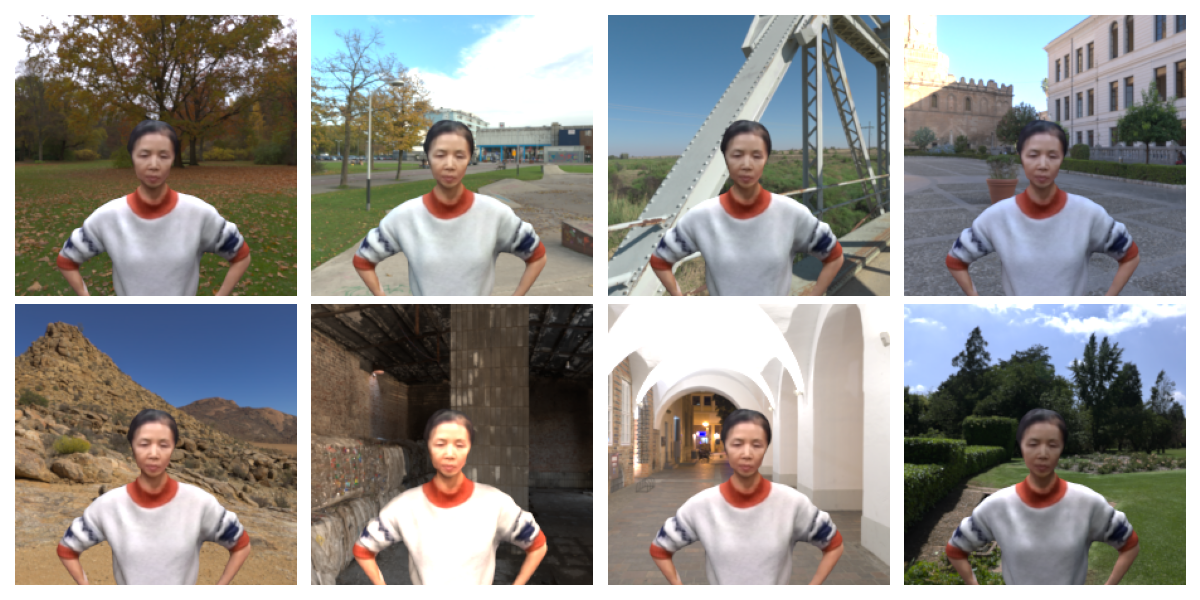
\includegraphics[scale=0.4]{imagenes/cap4/imagenes_fondos.png}
	\caption[Ejemplos de imágenes con diferentes fondos.]{Imágenes generadas con distintos fondos HDR.}
	\label{fig21.2}
\end{figure}

\begin{figure}[h]
	\centering
	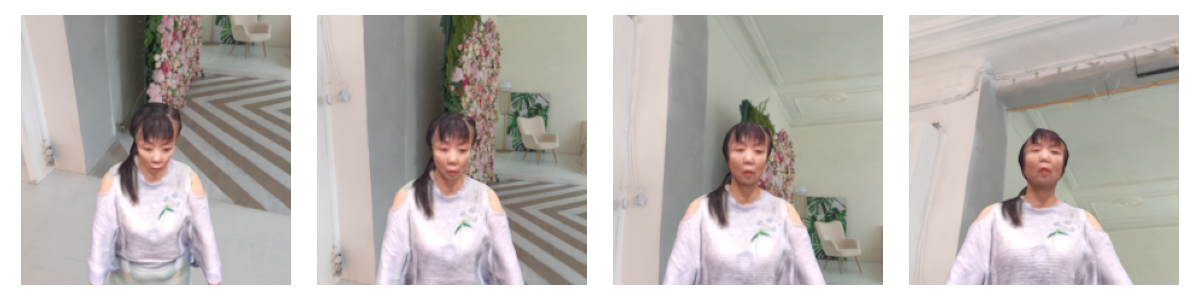
\includegraphics[scale=0.4]{imagenes/cap4/imagenes_rotacion_vertical2.png}
	\caption[Ejemplos de imágenes rotadas verticalmente.]{Imágenes generadas desde perspectivas más altas o más bajas. La secuencia se sigue de izquierda a derecha, mostrando rotaciones verticales que abarcan desde -30º hasta 30º en intervalos de 20º.}
	\label{fig22}
\end{figure}

\begin{figure}[h]
	\centering
	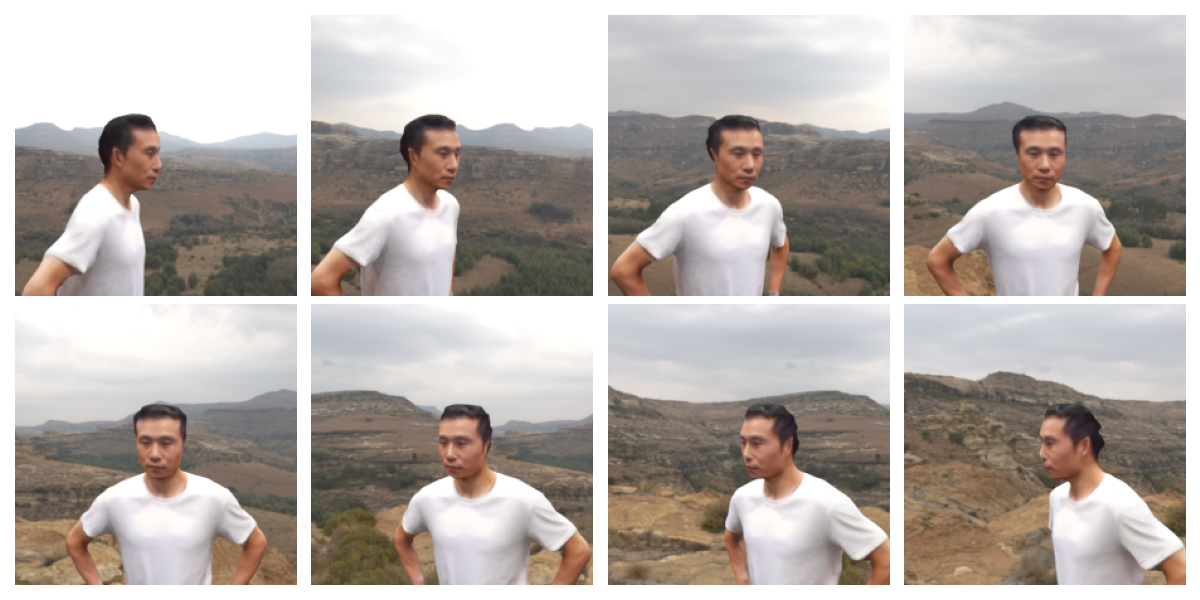
\includegraphics[scale=0.4]{imagenes/cap4/imagenes_rotacion_horizontal2.png}
	\caption[Ejemplos de imágenes rotadas horizontalmente.]{Imágenes generadas desde distintas perspectivas laterales. La secuencia se sigue de arriba hacia abajo y de izquierda a derecha, mostrando rotaciones horizontales que abarcan desde -70º hasta 70º en intervalos de 20º.}
	\label{fig23}
\end{figure}

Tras este proceso de generación de imágenes, y considerando que se contaba con 277 modelos 3D, el conjunto total de datos ascendió a 135730 imágenes. La gran diversidad de poses, expresiones faciales, modelos y fondos del conjunto de datos se pueden observar en la Figura \ref{fig24}.

% \begin{figure}[H]
% 	\centering
% 	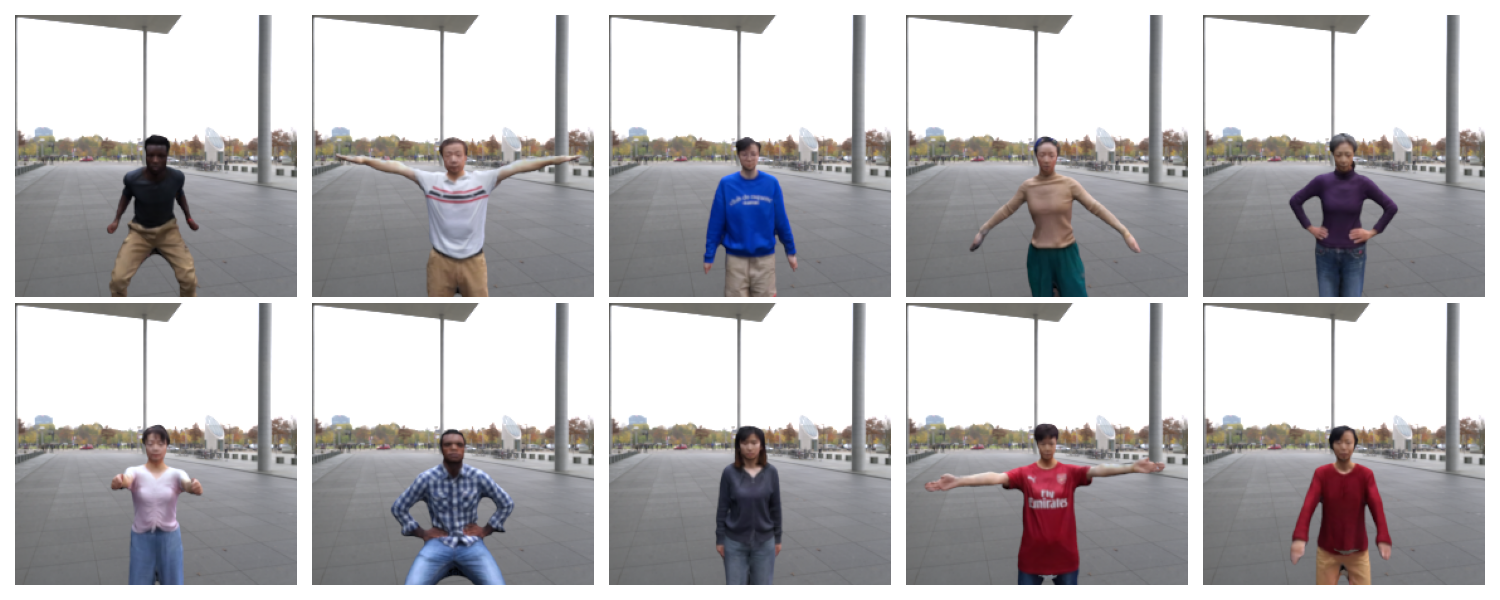
\includegraphics[scale=0.32]{imagenes/cap4/poses.png}
% 	\caption[Ejemplos de diversidad de poses.]{Imágenes que representan la diversidad de poses en el conjunto de datos.}
% 	\label{fig24.1}
% \end{figure}

\begin{figure}[h]
	\centering
	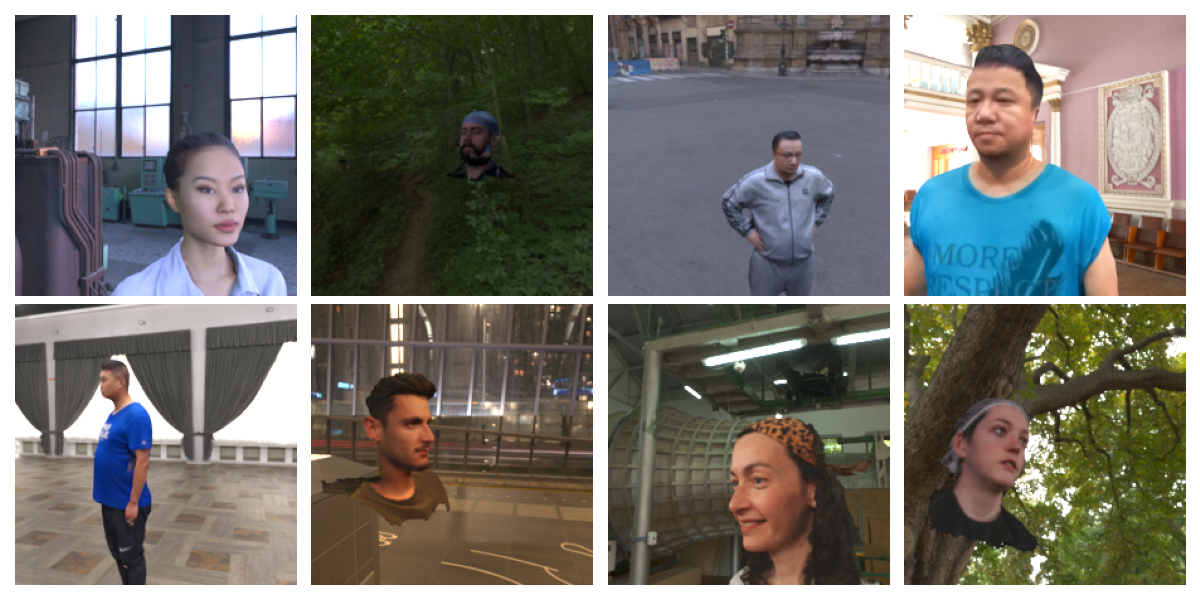
\includegraphics[scale=0.4]{imagenes/cap4/ejemplos_dataset.png}
	\caption[Ejemplos de imágenes generadas para el conjunto de datos.]{Imágenes generadas para el conjunto de datos sintético. Estos ejemplos contienen diferentes sujetos y distancias.}
	\label{fig24}
\end{figure}

\section{Métodos}

% Algo?

\subsection{FacialSCDnet}\label{fscdnet}

El método FacialSCDnet \cite{14}, es un enfoque de aprendizaje profundo para estimar la distancia entre el sujeto y la cámara en fotografías faciales. Se basa en una red neuronal convolucional, en concreto VGG-16 \ref{vgg16}, adaptada para regresar la distancia métrica de los individuos directamente desde las fotografías faciales. Este método consta de cuatro modelos de aprendizaje, uno por cada distancia focal presente en el conjunto de datos: 27 mm, 35 mm, 53 mm y 83.6 mm.

Para entrenar los modelos, se empleó un conjunto de datos compuesto por dos colecciones: 

\begin{itemize}
	\item Conjunto sintético: se generaron imágenes sintéticas 2D a partir de los modelos 3D de la base de datos Stirling ESRC 3D Face \footnote{Stirling ESRC 3D Face: https://pics.stir.ac.uk/ESRC/}. En particular, se utilizaron 315 modelos faciales de 54 individuos femeninos diferentes para generar aproximadamente 150.000 fotografías sintéticas.
	\item Conjunto de fotografías digitales: se adquirieron fotografías de 28 individuos siguiendo un protocolo de adquisición específico. Se consideraron 4 distancias focales diferentes (27 mm, 35 mm, 55 mm, 85 mm) en formato full frame y se capturaron 12 distancias diferentes de la cámara al sujeto, que oscilaron desde 50 cm hasta 6 m. Además, se fotografiaron 7 posiciones distintas de la cabeza, desde el perfil izquierdo hasta el perfil derecho, con intervalos de rotación de 30º. 
	% En la Figura \ref{fig24.25} se pueden ver algunas de las fotografías digitales. 
\end{itemize}

% \begin{figure}[H]
% 	\centering
% 	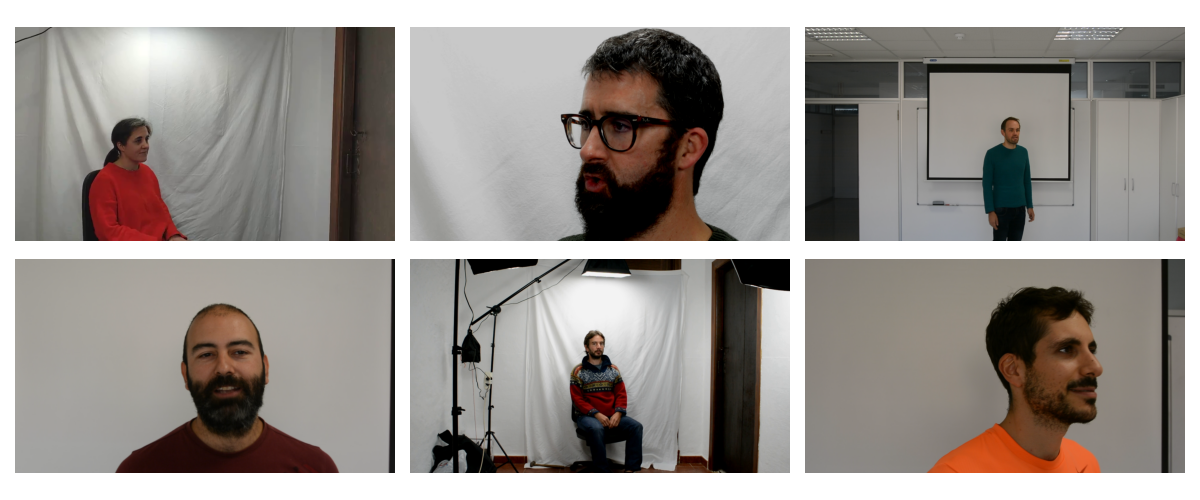
\includegraphics[scale=0.3]{imagenes/cap4/figura_FSCDnet_real.png}
% 	\caption[Ejemplos de imágenes reales FacialSCDnet.]{Imágenes adquiridas para la colección real de FacialSCDnet \cite{14}.}
% 	\label{fig24.25}
% \end{figure}

El proceso de entrenamiento de los modelos consta de dos fases. En primer lugar, se entrenan los modelos con el conjunto de datos sintéticos para capturar las relaciones entre la SCD y las características faciales. Posteriormente, se realiza un ajuste fino utilizando el conjunto de datos reales. Además, se aplica un proceso de aumento de datos que incluye la adición de diferentes fondos aleatorios a las imágenes (Figura \ref{fig24.2}), así como rotación, desenfoque, ruido, saturación, cambios de color e iluminación a las imágenes de entrenamiento.

\begin{figure}[h]
	\centering
	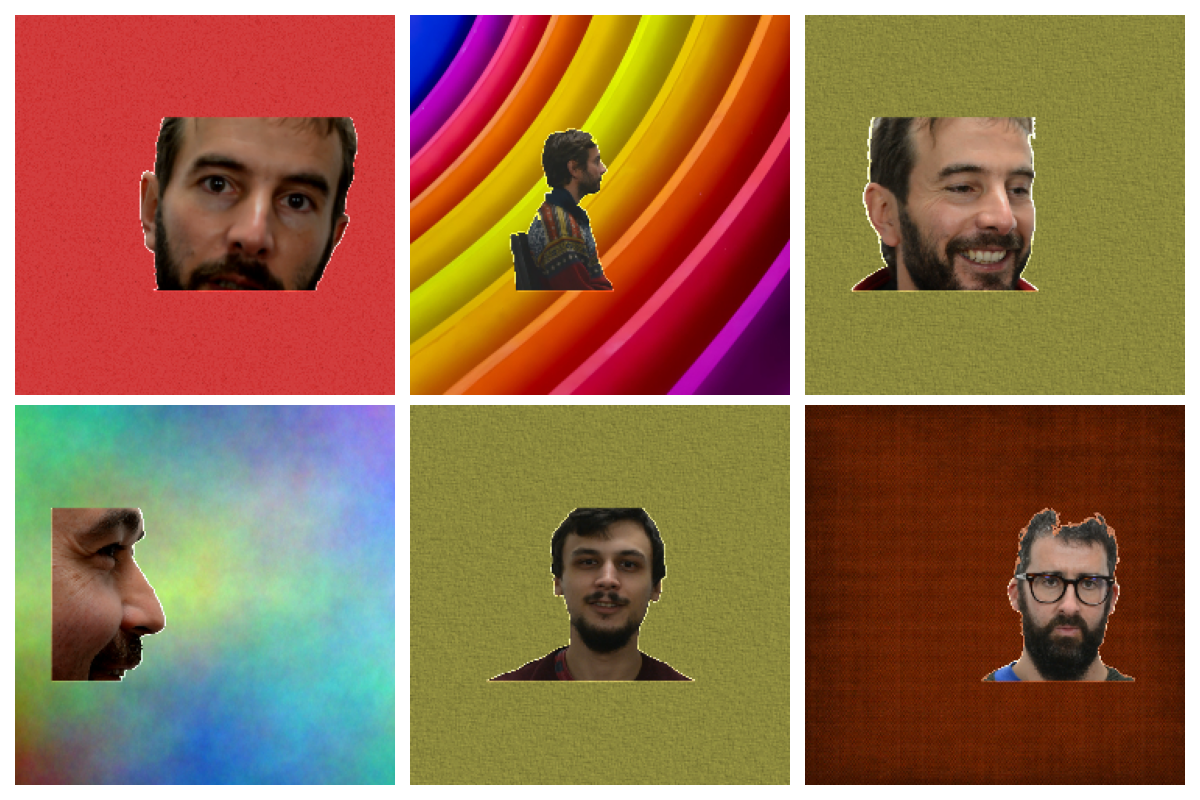
\includegraphics[scale=0.3]{imagenes/cap4/figura_FSCDnet.png}
	\caption[Ejemplos de imágenes reales con fondos FacialSCDnet.]{Imágenes reales con fondos utilizados en FacialSCDnet \cite{14}. Los rostros se integraron en los fondos aplicando una máscara con la silueta facial.}
	\label{fig24.2}
\end{figure}

A pesar de obtener resultados satisfactorios, este método presenta diversas limitaciones, entre las cuales destacan las siguientes: 

\begin{itemize}
	\item Sesgo del modelo con respecto al fondo: Las predicciones muestran una mejora significativa al introducir un fondo sintético en las imágenes originales, lo que indica una dependencia del modelo con este aspecto. Esta tendencia sugiere una limitada capacidad de generalización, dado que las imágenes con el fondo original obtienen un rendimiento inferior en las predicciones en comparación con aquellas con fondo sintético.
	\item Limitación del conjunto de datos: La colección sintética consta de una única base de datos facial que está compuesta exclusivamente por individuos femeninos. Además, la colección real incluye un número reducido de individuos.
	\item Eficiencia del \textit{framework}: La implementación del método en \textit{Keras}, si bien popular, se ve afectada por su relativa lentitud en comparación con otros \textit{frameworks} para trabajar con arquitecturas de \textit{deep learning}.
\end{itemize}

\subsection{FacialSCDnet+}

El método FacialSCDnet+, basado en FacialSCDnet \ref{fscdnet}, es un enfoque mejorado para estimar la distancia entre el sujeto y la cámara en fotografías faciales. Este método presenta dos modelos de aprendizaje: uno basado en la arquitectura VGG-16 y otro en la arquitectura ResNet-50, ambos adaptados para regresar la SCD. Estos modelos fueron entrenados para predecir en imágenes con una distancia focal aproximada de 35 mm.

A diferencia de FacialSCDnet, este método emplea un conjunto de datos completamente sintético, el cual es considerablemente más realista, diverso y extenso en comparación con su predecesor. Además, se ha rediseñado el sistema de aumento de imágenes aplicando las operaciones siguientes:

\begin{itemize}
	\item Transformaciones afines: Se aplican rotaciones aleatorias de hasta 15 grados en sentido horario o antihorario, así como traslaciones horizontales y verticales de hasta el 20\% del tamaño de la imagen, con una probabilidad del 100\%. Esta transformación simula diferentes perspectivas de las imágenes.
	\item Emborronado Gaussiano: Se aplica un emborronado gaussiano con un \textit{kernel} de tamaño 1 y un sigma aleatorio entre 0.1 y 2.0, lo que suaviza la imagen, con una probabilidad del 25\%. Esta transformación ayuda a introducir algo de ruido en las imágenes.
	\item Nitidez: Se ajusta la nitidez de la imagen aplicandole un factor de nitidez de valor 2, con una probabilidad del 25\%. Esta transformación simula una mejor definición de las imágenes
	\item Alteraciones de color: Se aplican ajustes aleatorios en el brillo, contraste y tono de la imagen, con un rango de variación entre $\pm$ 0.1 en cada canal, con una probabilidad del 25\%. Esta transformación contribuye a aumentar la diversidad en la apariencia de las imágenes.
	\item Borrado de píxeles: Se borran zonas de píxeles aleatorias de la image. Estas zonas tienen un tamaño de entre el 2\% y el 5\% de la imagen, y la relación de aspecto está entre un 0.5 y un 1.5, dotando a estas zonas de un aspecto más rectangular. Esta transformación tiene una probabilidad del 25\%. Esta transformación introduce un grado adicional de variabilidad y robustez frente a la ocultación parcial de información.
	\item Escala de grises: La imagen se convierte a escala de grises, perdiendo la información de color, con una probabilidad del 25\%. Esta transformación permite al modelo mejorar su invarianza al color.
\end{itemize}

Estas nuevas transformaciones aumentan la calidad del conjunto de datos de entrenamiento, mejorando la robustez y la capacidad de generalización del modelo ante diferentes condiciones y variaciones en las imágenes de entrada.

\begin{figure}[h]
	\centering
	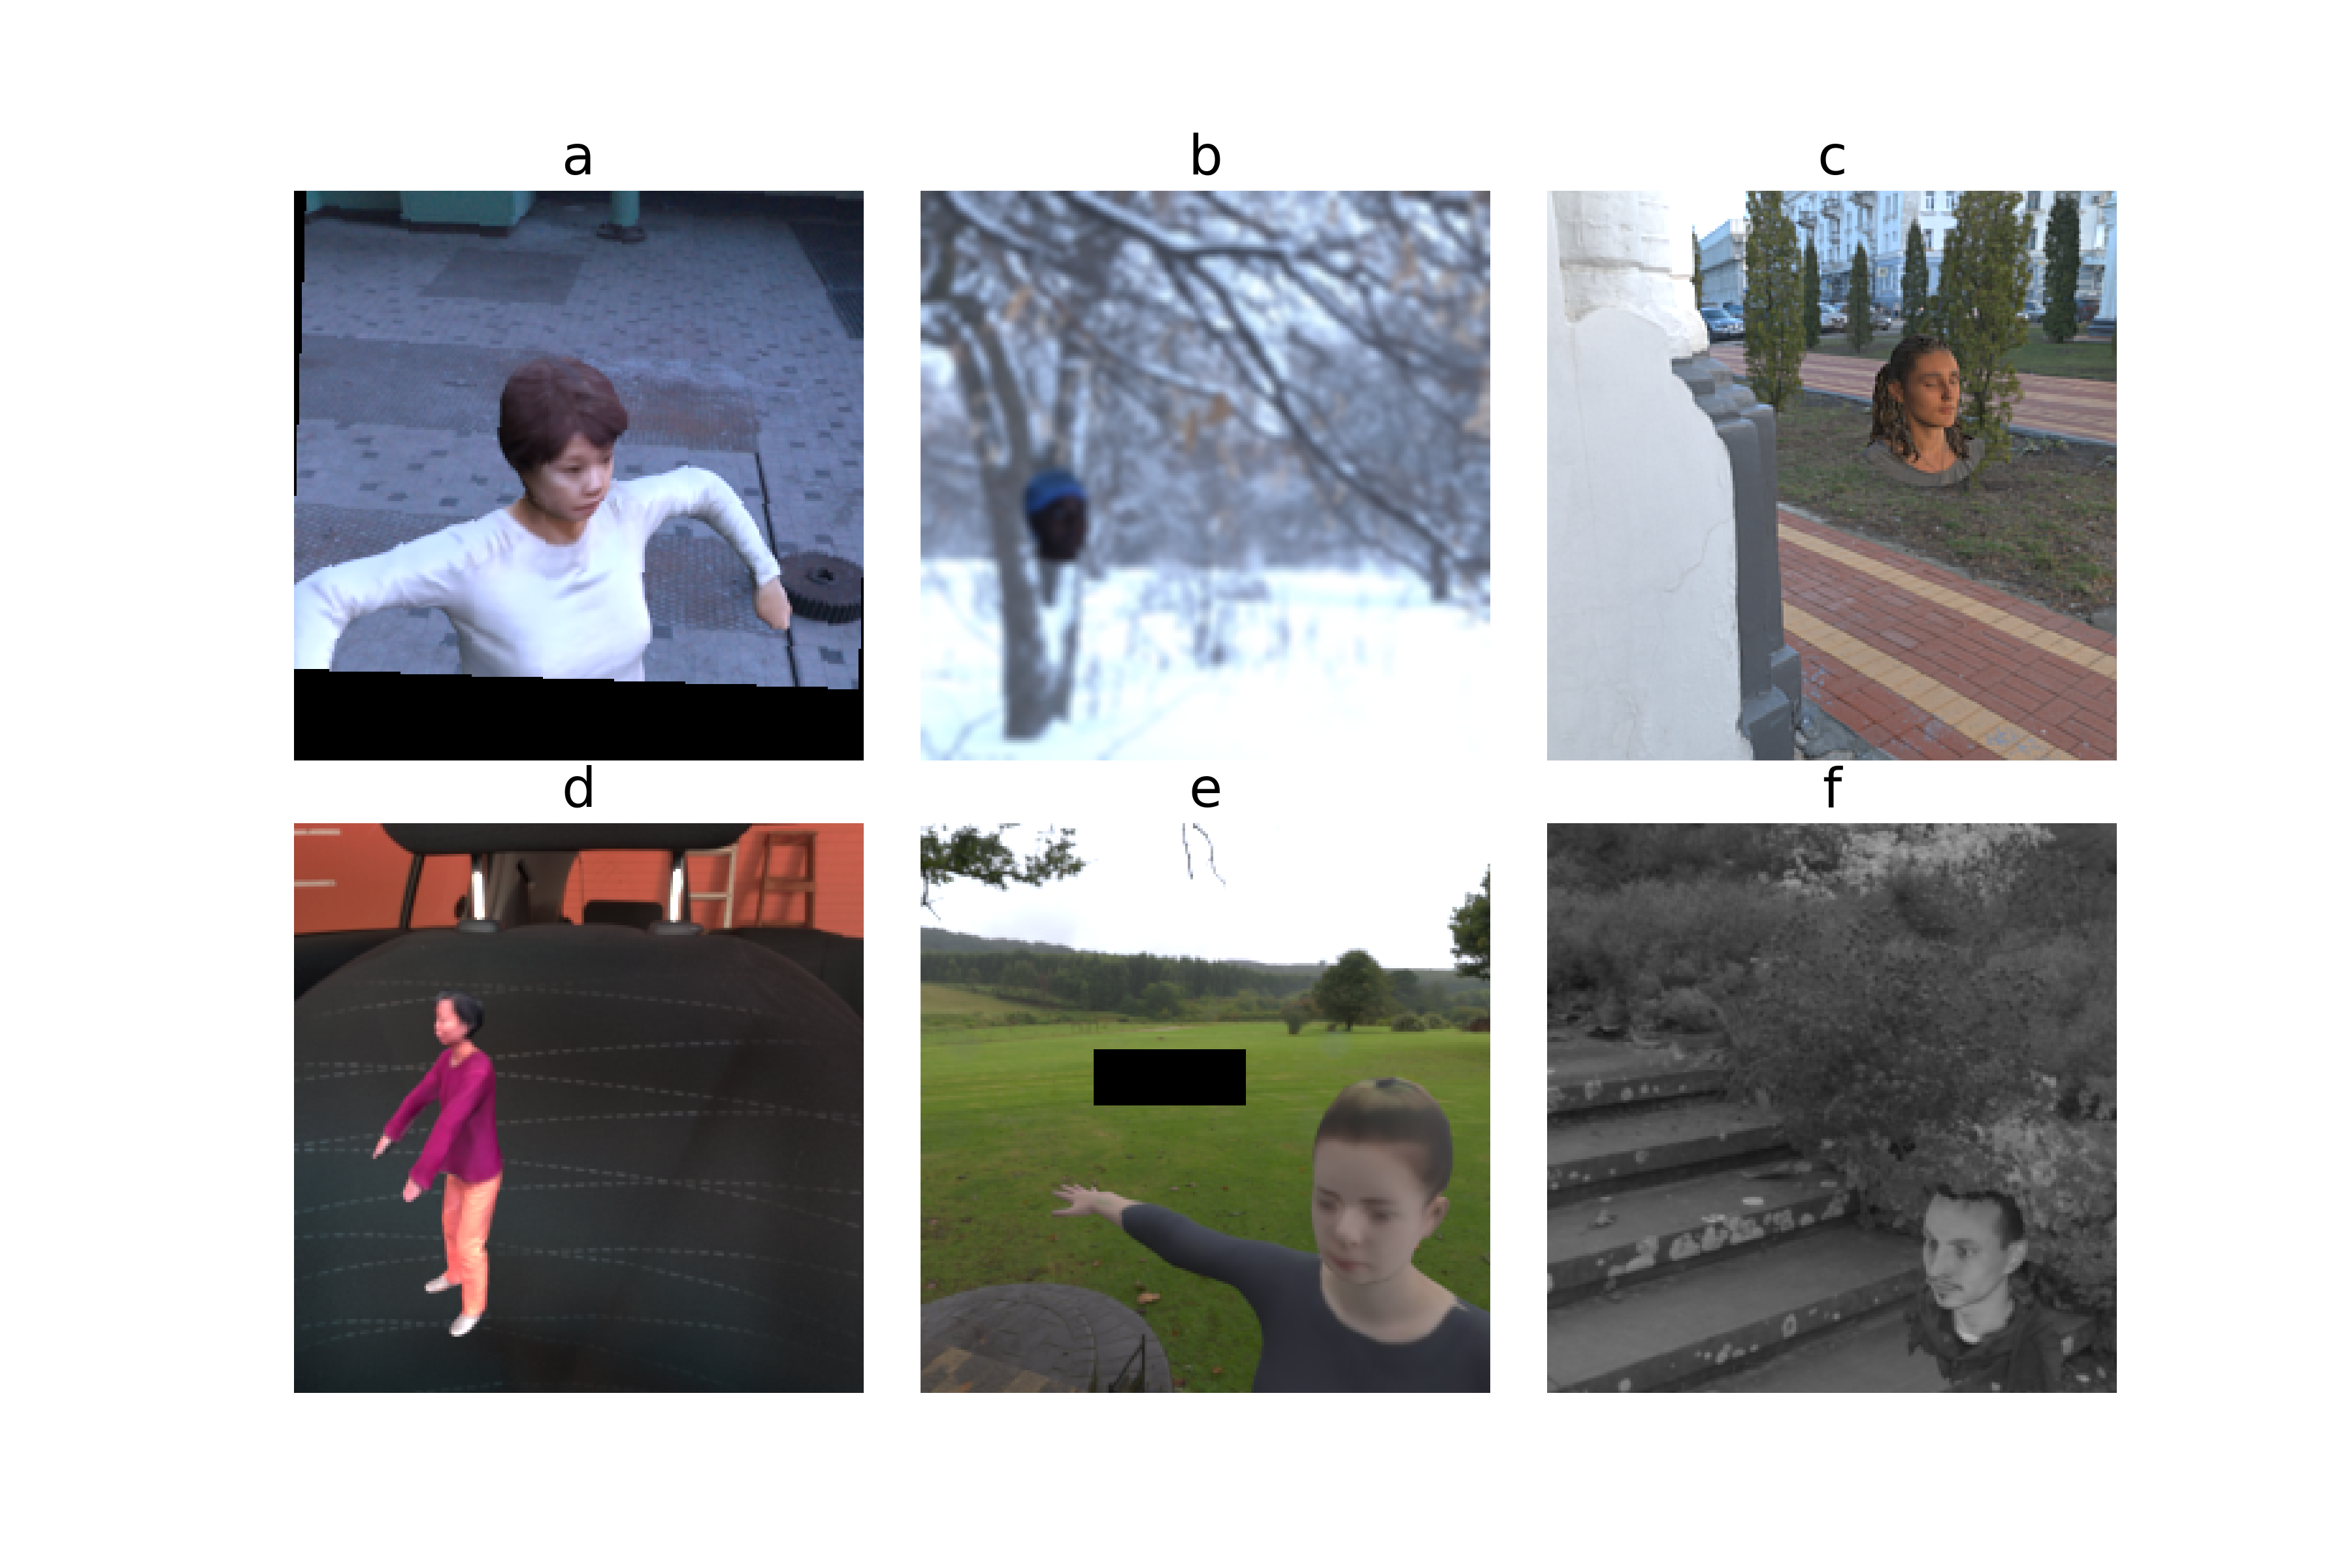
\includegraphics[scale=0.4]{imagenes/cap4/augmented_images.png}
	\caption[Transformaciones utilizadas en el aumento de datos.]{Transformaciones aplicadas a las imágenes: a) transformaciones afines, b) emborronado gaussiano, c) nitidez, d) alteraciones de color, e) borrado de píxeles, f) escala de grises.}
	\label{fig25}
\end{figure}

A continuación, se detallaran los aspectos técnicos de implementación más relevantes, junto con el diseño experimental del método.

\subsubsection{Gestión de experimentos}

En el método FacialSCDnet+ se ha puesto en práctica la metodología MLOps. Esta metodología ha surgido como una respuesta efectiva para mejorar la gestión de experimentos en el campo del aprendizaje automático. Al implementar MLOps, se persigue un doble objetivo: automatizar y monitorizar de manera eficiente los procesos relacionados con el desarrollo, entrenamiento y despliegue de modelos de ML, a la vez que se garantiza la coherencia y reproducibilidad de los resultados obtenidos en todo momento. Este enfoque integral no solo aumenta la eficiencia y la fiabilidad de los sistemas de IA, sino que también fomenta una cultura de colaboración, transparencia y mejora continua en los equipos de desarrollo y operaciones.

Para llevar a cabo esta metodología, se ha hecho uso de la librería \textit{MLflow}, una herramienta que facilita la gestión y el seguimiento del proceso de desarrollo de modelos de aprendizaje automático. Esta librería no solo proporciona un entorno unificado para organizar experimentos y compartir resultados, sino que también ofrece capacidades avanzadas de seguimiento y visualización de métricas, parámetros y artefactos asociados con cada iteración del proceso de desarrollo.

\subsubsection{Optimización de hiperparámetros}

El ajuste de hiperparámetros es esencial en el desarrollo de modelos de ML, ya que éstos controlan el comportamiento y la complejidad del algoritmo de aprendizaje. La optimización adecuada puede mejorar significativamente el rendimiento del modelo en términos de precisión, velocidad de entrenamiento y capacidad de generalización. Además, el proceso de ajuste de hiperparámetros permite explorar el espacio de búsqueda de manera sistemática, lo que proporciona una comprensión más profunda del comportamiento del modelo y sus interacciones con los datos.

Con el objetivo de realizar la optimización de hiperparámetros, se ha optado por utilizar \textit{Optuna}, una librería de optimización de hiperparámetros automatizada. Esta herramienta ofrece una manera eficiente de encontrar los mejores valores para los hiperparámetros de un modelo de aprendizaje automático. En particular, se emplea el algoritmo conocido como \textit{Tree-structured Parzen Estimator} (TPE) \cite{71}, el cual es una técnica de muestreo que ajusta una distribución probabilística a los datos recopilados durante la búsqueda para dirigir la exploración hacia regiones prometedoras del espacio de búsqueda. Además, se utiliza una técnica de poda para descartar de manera temprana las configuraciones de hiperparámetros menos prometedoras, lo que contribuye a acelerar el proceso de búsqueda y mejorar su eficiencia.


\subsubsection{Cambio de \textit{framework}}

El método FacialSCDnet fue desarrollado utilizando \textit{Keras}, uno de los principales \textit{frameworks} en \textit{deep learning}. \textit{Keras} es una biblioteca de código abierto que fue adoptada e integrada en \textit{Tensorflow} a mediados de 2017. A pesar de su popularidad, \textit{Keras} está escrita en alto nivel, lo que implica una mayor facilidad de uso pero un menor rendimiento en cuanto a velocidad. Esta biblioteca es una excelente opción para conjuntos de datos pequeños o prototipos rápidos, ya que permite construir, entrenar y evaluar modelos de manera rápida. Sin embargo, debido al gran volumen de datos y experimentos en este proyecto, \textit{Keras} puede quedarse rezagado en cuanto a rendimiento.

Por esta razón, en FacialSCDnet+ se modifica el \textit{framework} utilizado. En concreto, se realiza una transición desde la versión 1.15 de \textit{TensorFlow}, desarrollada en 2019, a la versión 2.0.1 de \textit{PyTorch}, lanzada en 2023. Esta librería, relativamente reciente, cuenta con un excelente soporte comunitario y un desarrollo activo. Entre sus principales ventajas se incluyen:

\begin{itemize}
	\item Flexibilidad: \textit{PyTorch} ofrece un control más granular sobre cada aspecto del modelo gracias a su API de bajo nivel.
	\item Simplicidad: A pesar de su bajo nivel de operación, \textit{PyTorch} se siente natural, lo que facilita la programación y la hace más intuitiva.
	\item Depuración: \textit{PyTorch} facilita la depuración de modelos gracias a su estructura dinámica de grafos computacionales, lo que permite una mejor visualización y seguimiento de errores.
	\item Eficiencia en el uso de memoria: \textit{PyTorch} optimiza el uso de memoria a través de técnicas como la gestión de tensores y el cálculo diferencial automático, permitiendo un uso más eficiente de los recursos disponibles.
\end{itemize}


\subsubsection{Protocolo de validación experimental}\label{protocolo}

La técnica empleada para llevar a cabo el entrenamiento se conoce como \textit{hold-out} (Figura \ref{fig27}). Esta metodología implica dividir el conjunto de datos en dos partes distintas: el conjunto de entrenamiento y el conjunto de test. A su vez, dentro del conjunto de entrenamiento, se realiza una subdivisión adicional para crear un conjunto de validación. Este conjunto se utiliza durante el proceso de entrenamiento del modelo para evaluar periódicamente la calidad del mismo mediante comparaciones con las métricas obtenidas en el conjunto de entrenamiento. Una vez finalizado el entrenamiento, se evalúa el modelo utilizando el conjunto de test, que contiene datos que no se han visto nunca durante el entrenamiento, con el propósito de obtener una evaluación definitiva sobre la calidad del aprendizaje.

\begin{figure}[H]
	\centering
	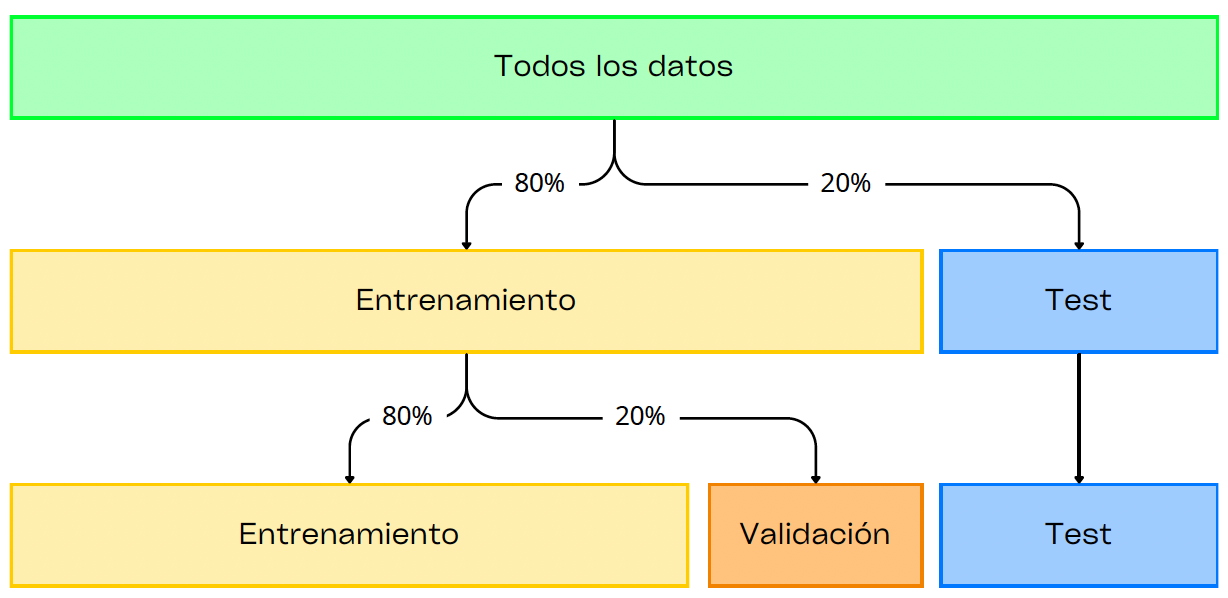
\includegraphics[scale=0.55]{imagenes/cap5/hold-out.png}
	\caption[Esquema de división del conjunto de datos.]{Esquema de división del conjunto de datos total en los subconjuntos de entrenamiento, validación y test.}
	\label{fig27}
\end{figure}

El primer paso consiste en reservar todas las imágenes de 30 sujetos de forma aleatoria para el conjunto de test. Posteriormente, se añaden imágenes adicionales de manera aleatoria, para constituir el 20\% del conjunto total de test, mientras que el 80\% restante se asigna al conjunto de entrenamiento.

Finalmente, durante el proceso de entrenamiento de los modelos, se aparta un 20\% aleatorio del conjunto de entrenamiento como conjunto de validación, dejando el 80\% restante para el entrenamiento propiamente dicho. Por tanto, contamos con 135730 imágenes, de las cuales 85435 se destinan al entrenamiento, 21360 a la validación y 28935 a test.


\subsubsection{Métricas}

Dado que se aborda un problema de regresión en el que la importancia de la distorsión a distancias cercanas es crucial, se ha optado por emplear la distorsión como función de pérdida. Esta medida se calcula mediante la siguiente fórmula:

\begin{equation}
	\text{Distorsion} = \displaystyle \frac{\sum_{i=1}^{n} | \displaystyle \frac{1}{1 + \displaystyle \frac{y_i}{d}} - \displaystyle \frac{1}{1 + \displaystyle \frac{x_i}{d}}|}{n}
\end{equation}

siendo $y_i$ la distancia verdadera en la imagen $i$, $x_i$ la distancia predicha en la imagen $i$, y $d = 12.6572 $ cm, que corresponde a un valor derivado de cálculos geométricos \cite{55} para obtener experimentalmente el factor de distorsión de una cabeza humana de tamaño promedio, según la SCD de la fotografía.

Esta función de pérdida asegura que el modelo aprenda a predecir distancias cercanas con mayor precisión, mitigando así la posibilidad de una distorsión significativa.

Aunque la distorsión se considera la medida principal de rendimiento, también se han empleado otras métricas como el error absoluto medio (MAE) y el error relativo medio (MRE) para evaluar el desempeño del modelo:

\begin{equation}
	\text{MAE} = \frac{1}{n} \sum_{i=1}^{n} | y_i - x_i |
\end{equation}

\begin{equation}
	\text{MRE} = \frac{1}{n} \sum_{i=1}^{n} \frac{| y_i - x_i |}{y_i}
\end{equation}

El MAE, al calcular la diferencia absoluta promedio entre las predicciones del modelo y los valores reales, mide cuánto se desvían las predicciones del modelo en términos absolutos. Esto es útil para entender la magnitud de los errores de predicción sin considerar su distorsión.
Por otro lado, el MRE, al calcular la diferencia relativa promedio entre las predicciones del modelo y los valores reales, proporciona una medida de cuánto se desvían las predicciones del modelo en relación con la distancia real (normalmente en porcentaje). Esto es fundamental cuando se necesita evaluar el rendimiento del modelo en términos de precisión relativa.

\subsection{\textit{Backend}}\label{backend}

\subsubsection{VGG-16}\label{vgg16}

VGG-16 es una red neuronal convolucional profunda basada en la arquitectura VGGNet \cite{65}. Esta red contiene 16 capas entrenables, como su nombre indica, y destaca por su eficacia en la extracción de características en imágenes.

La arquitectura VGG-16 se puede ver en la Figura \ref{fig26}. Inicialmente, la red recibe como entrada una imagen RGB de tamaño fijo de 224x224. Esta imagen atraviesa una serie de capas convolucionales, donde se emplean filtros de tamaño 3x3. En estas capas, el \textit{stride} se mantiene constante en 1 píxel y se utiliza un \textit{padding} de 1 píxel para evitar la pérdida de dimensionalidad al aplicar los filtros de convolución 3x3. Cada capa convolucional contiene una capa de activación ReLU detrás.Tras algunas de las capas convolucionales, se realiza un \textit{max pooling} con filtros de 2x2 y \textit{stride} de 2 píxeles, esta operación se realizar para ir reduciendo el tamaño de los mapas de activación. En esta primera parte de la red es donde se extraen las características de la imagen.

Posteriormente, esta primera parte de la red es sucedida por tres capas totalmente conectadas: las dos primeras cuentan con 4096 neuronas cada una, mientras que la tercera realiza la clasificación con 1000 neuronas (una por cada clase). Tras cada una de estas capas, sigue una capa de activación ReLU. La última capa corresponde a la capa de \textit{soft-max} que calcula las probabilidades de pertenecer a cada clase. En esta parte final de la red se realiza la clasificación final de las características extraídas para la tarea de reconocimiento de imágenes.

\begin{figure}[h]
	\centering
	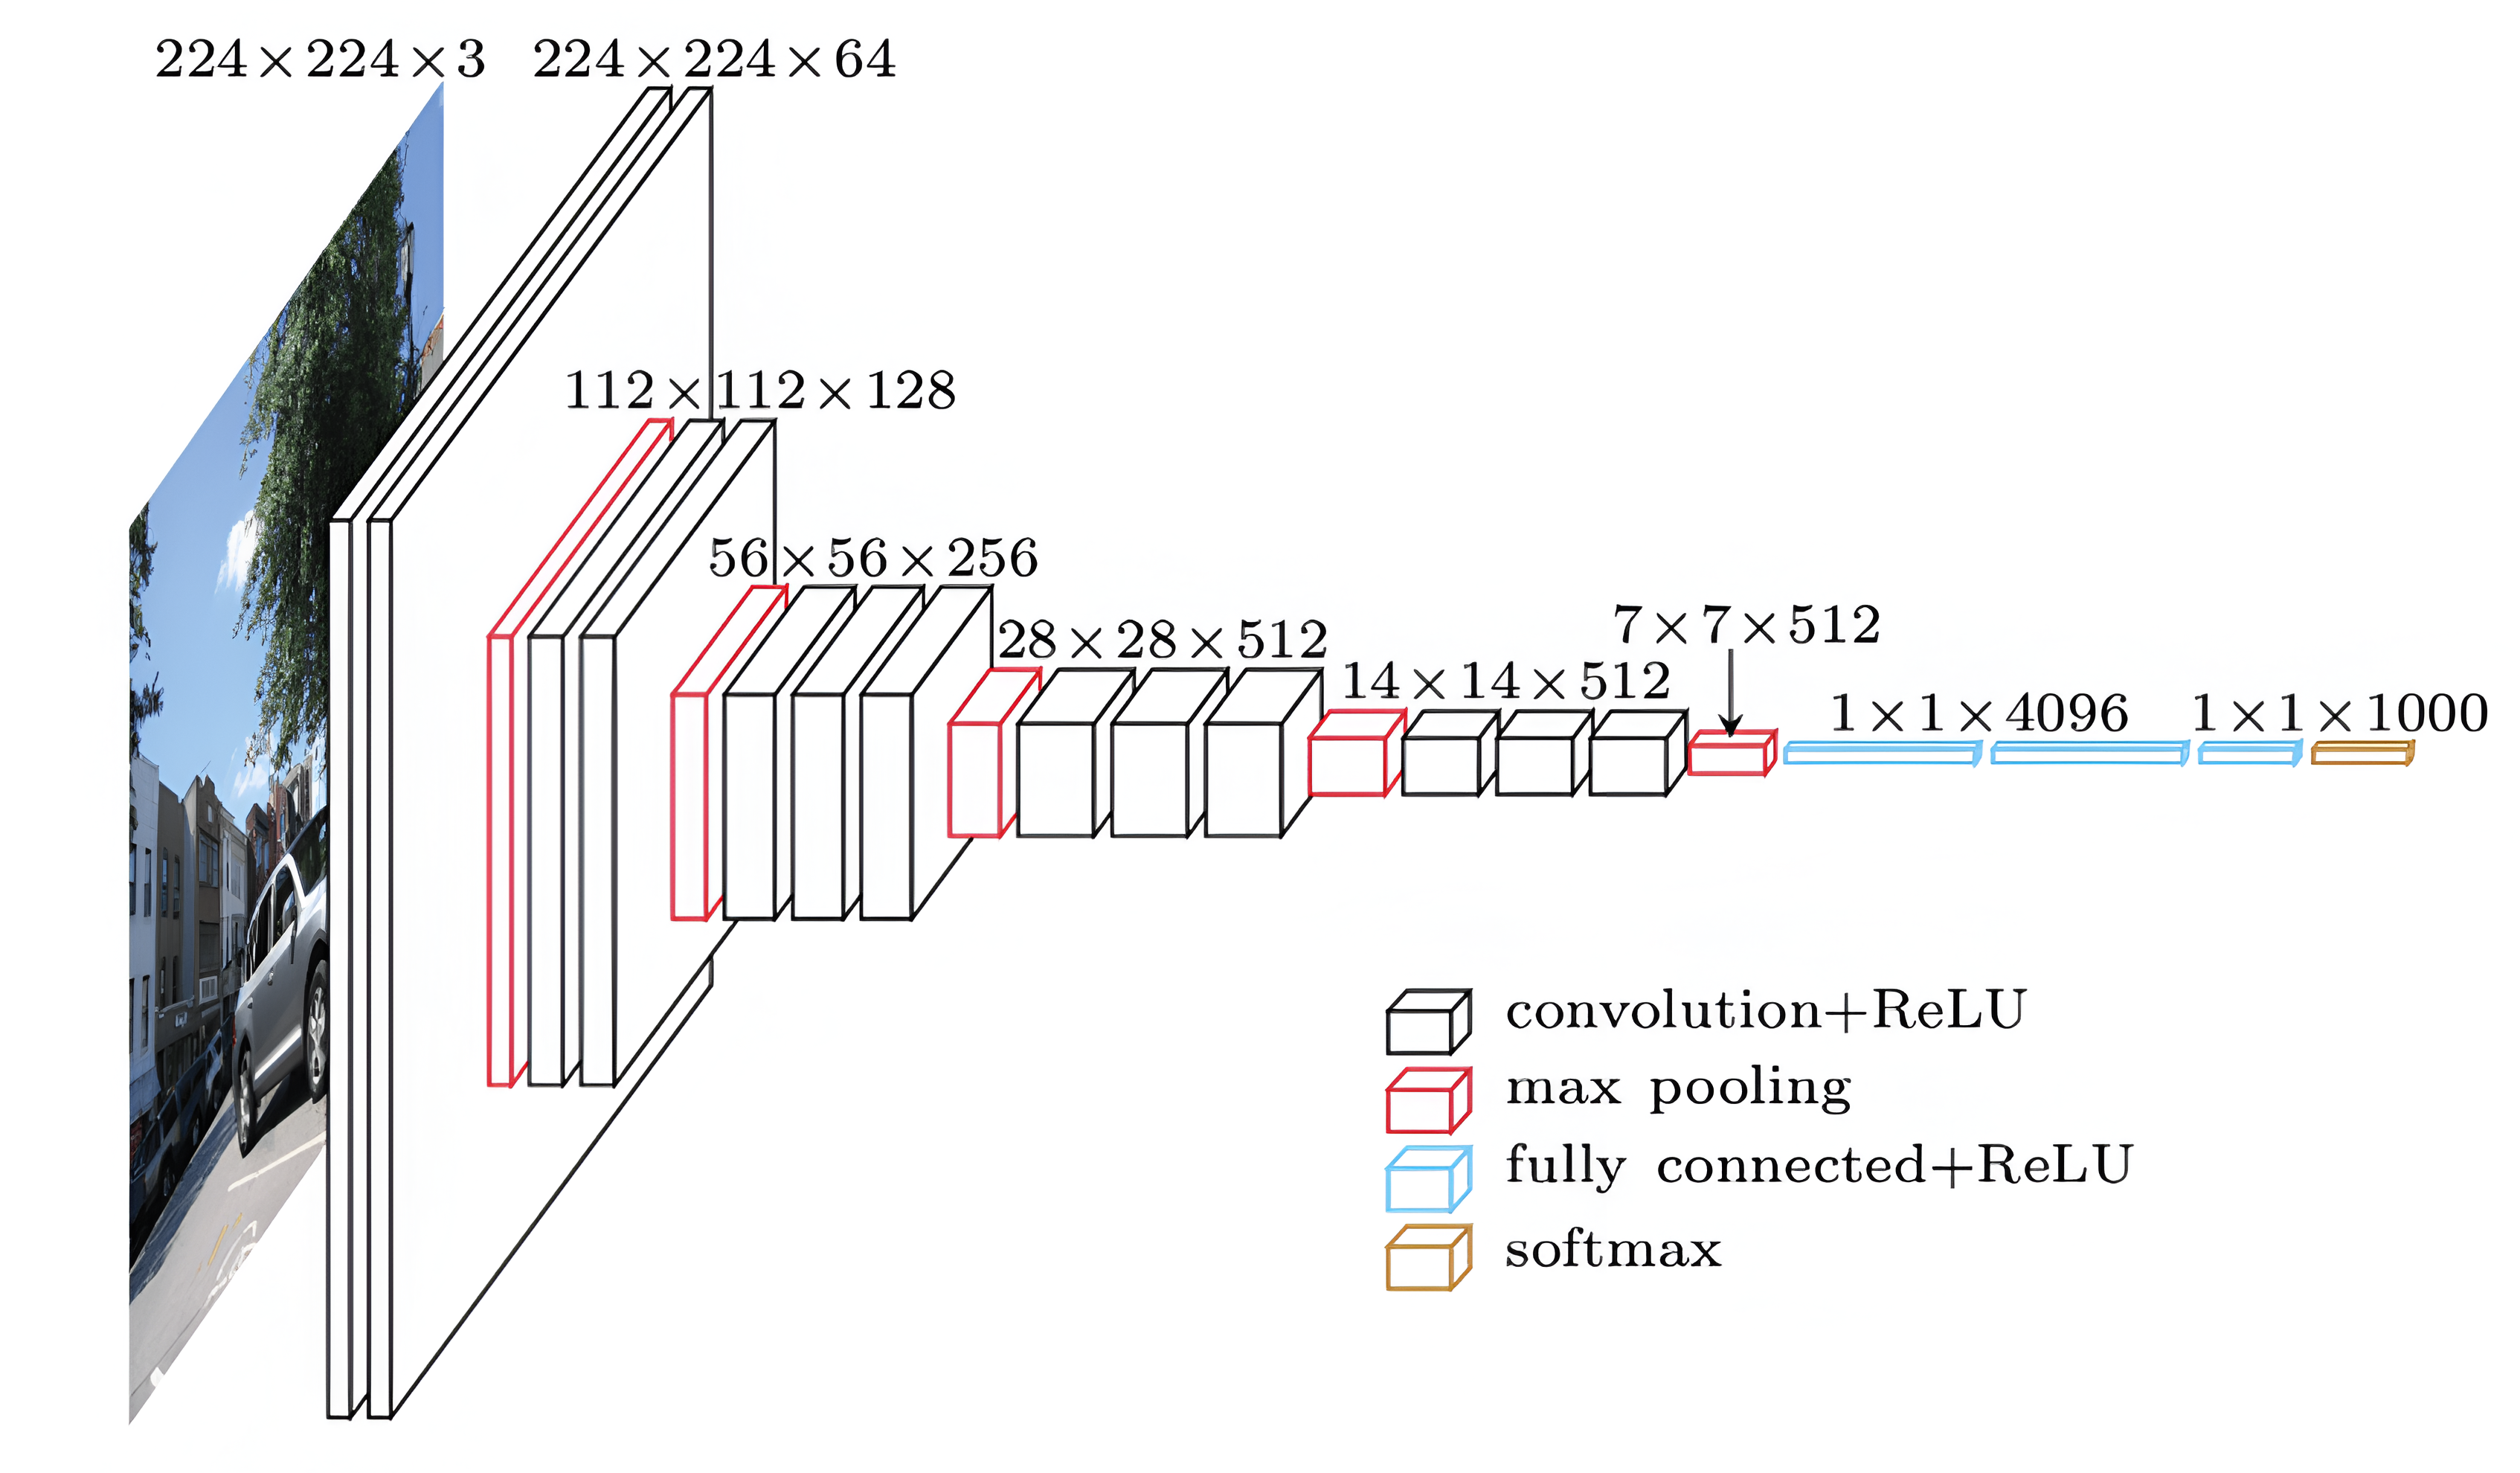
\includegraphics[scale=0.1]{imagenes/cap4/vgg-16.png}
	\caption[Arquitectura de la red VGG-16.]{Arquitectura de la red VGG-16. Las dimensiones se muestran en formato: Columnas x Filas x Canales \cite{66}.}
	\label{fig26}
\end{figure}

Las arquitecturas VGGnet destacan por emplear convoluciones únicamente de tamaño 3x3. Este enfoque representó un importante avance con respecto a las arquitecturas predecesoras, ofreciendo diversas ventajas significativas:

\begin{itemize}
	\item Mayor profundidad: Permite aplicar más convoluciones e incrementar la profundidad de la red al tener menos parámetros entrenables.
	\item Agregación implícita de escalas: Combinando las pequeñas convoluciones y la profundidad de la red, se pueden detectar características a pequeña escala, mientras que la agregación de escalas mayores va implícita al pasar de capa.
\end{itemize}

En FacialSCDnet y FacialSCDnet+, se realizó una modificación estructural en la red originalmente diseñada para clasificación. Se mantuvo la extracción de características a través de los 5 bloques convolucionales, aprovechando los pesos preentrenados en ImageNet \footnote{ImageNet: https://www.image-net.org/}. Sin embargo, se eliminó la parte superior de la red y se agregaron 2 capas totalmente conectadas de 4096 neuronas, junto con una capa final de una neurona configurada para llevar a cabo la tarea de regresión.

Tras realizar estos ajustes en la estructura de la red, se congelaron los pesos de los bloques convolucionales, mientras que la parte final de la red se entrenó desde cero. En total, la red cuenta con 119,545,857 parámetros para el entrenamiento.

El uso de esta red se justifica por su sencillez y su capacidad para aprender características significativas de las imágenes mediante el bloque de capas convolucionales. Dado su alto número de parámetros a entrenar, VGG-16 demanda recursos computacionales significativos, sin embargo, su gran rendimiento en el procesamiento de imágenes lo convierte en una opción atractiva para este trabajo.

\subsubsection{ResNet-50}

ResNet-50 es una red neuronal convolucional profunda que pertenece a la familia de las redes residuales \cite{72} (ResNets). Estas redes destacan por la introducción de conexiones \enquote*{residuales}, diseñadas para evitar el desvanecimiento del gradiente, uno de los principales problemas de las CNN profundas.
Este problema surge durante el entrenamiento de las redes neuronales cuando se emplean métodos basados en descenso estocástico de gradientes y retropropagación. En concreto, ocurre cuando los gradientes de la función de error con respecto a los pesos de la red se vuelven excesivamente pequeños, lo que dificulta la actualización de dichos pesos durante el proceso de aprendizaje. Esta situación puede interrumpir el aprendizaje, especialmente en redes profundas con múltiples capas.

En las ResNets, en lugar de simplemente apilar capas una sobre otra, se añaden conexiones directas que saltan una o más capas (Figura \ref{fig28}). Estas conexiones de atajo permiten que la red aprenda las diferencias entre la representación deseada y la representación actual, en lugar de tener que aprender la representación completa en cada capa. Este enfoque permite aumentar la profundidad de la red sin que su rendimiento se vea afectado.

\begin{figure}[h]
	\centering
	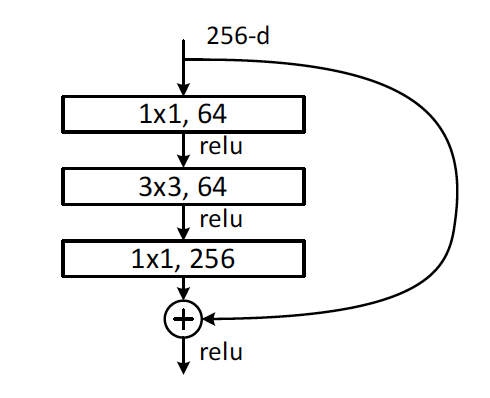
\includegraphics[scale=0.65]{imagenes/cap4/residual_conections.png}
	\caption[Bloque residual ResNet.]{Bloque \textit{bottleneck} construido para las ResNet-50/101/152 \cite{73}. Este bloque consiste en tres capas de convolución: una convolución 1x1 que reduce la dimensionalidad a 64 canales, seguida de una convolución 3x3, que aprende las características espaciales, y otra convolución 1x1 que restaura la dimensionalidad original de 256 canales. Todas las capas de convolución usan activaciones ReLU. La conexión de salto agrega la entrada del bloque directamente a la salida, antes de pasar por una activación ReLU final.}
	\label{fig28}
\end{figure}

La arquitectura ResNet-50 se puede observar en la Figura \ref{fig29}. Esta consta de 50 capas, incluyendo capas convolucionales, capas de \textit{pooling} y capas totalmente conectadas. Inicialmente, la imagen de entrada se procesa a través de una capa de convolución seguida de una capa de agrupamiento. A esta capa le siguen varias capas de bloques residuales, cada uno de ellos consta de múltiples capas de convolución

\begin{itemize}
	\item Entrada: La imagen de entrada se procesa inicialmente a través de una capa de convolución seguida de una capa de agrupamiento promedio.
	\item Bloques de convolución: ResNet-50 tiene varias capas de bloques residuales. Estos bloques se repiten varias veces, y cada uno consta de múltiples capas de convolución. Aquí es donde se incorporan las conexiones \enquote*{residuales}, la entrada de cada bloque se añade a la salida del bloque.
	\item Capa de \textit{pooling}: Tras los bloques convoluciones hay una capa de agrupamiento máximo.
	\item Capas totalmente conectadas: Por último, las características se pasan a un vector unidimensional y se conectan a través de una capa totalmente conectada para generar las predicciones finales.
\end{itemize}

\begin{figure}[h]
	\centering
	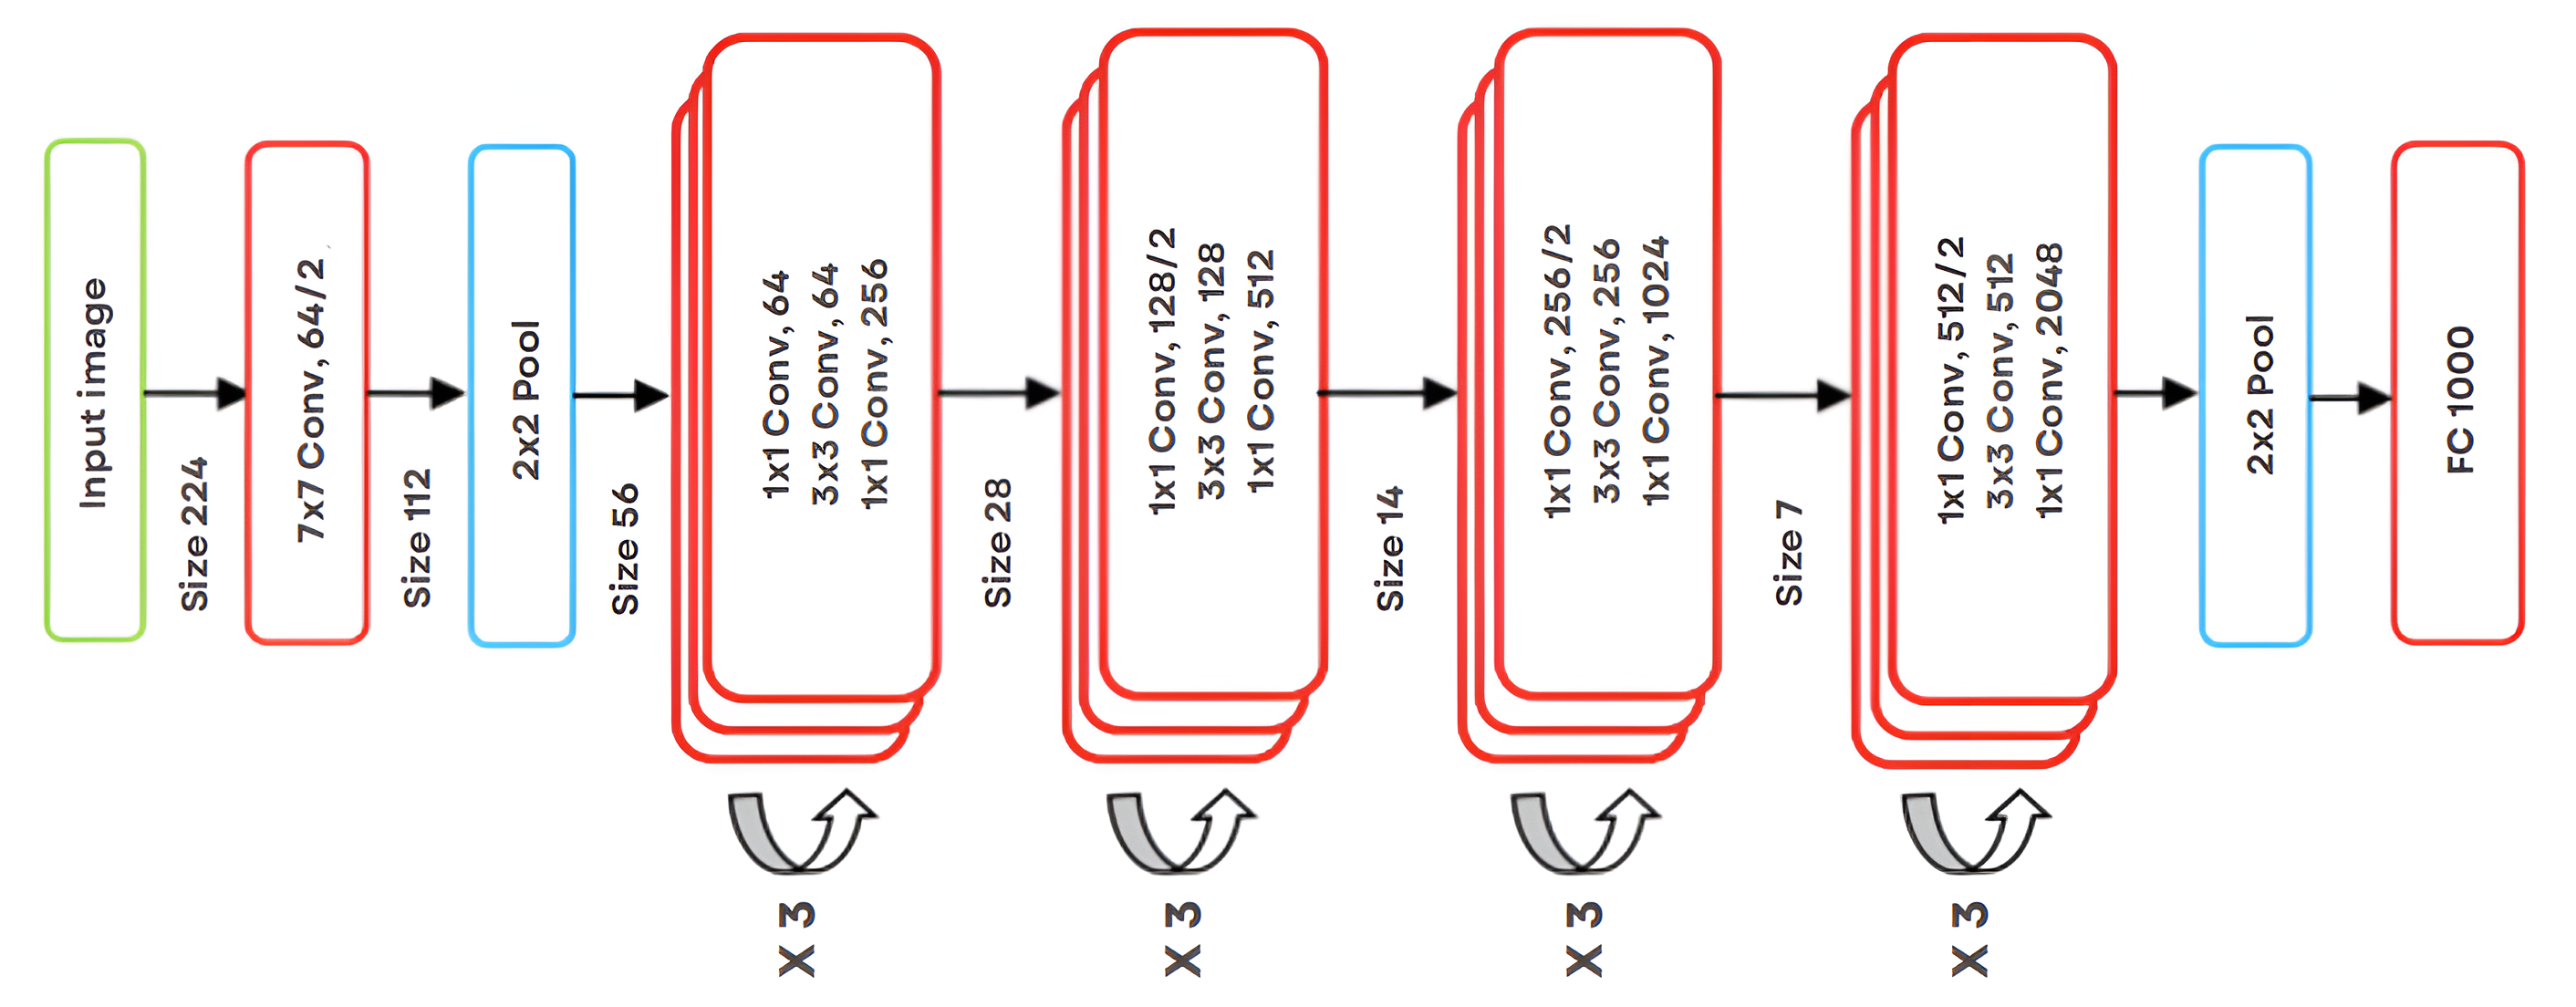
\includegraphics[scale=0.12]{imagenes/cap4/resnet.png}
	\caption[Arquitectura de la red ResNet-50.]{Arquitectura de la red ResNet-50 \cite{73}.}
	\label{fig29}
\end{figure}

En FacialSCDnet+, al igual que con VGG-16, se realizó una modificación estructural en la red originalmente diseñada para clasificación. Se mantuvo la extracción de características a través de los bloques residuales, aprovechando los pesos preentrenados en ImageNet. Sin embargo, se prescindió de la última capa de la red y se agregaron 2 capas totalmente conectadas de 4096 neuronas, junto con una capa final de una neurona configurada para llevar a cabo la tarea de regresión.

Tras realizar estos ajustes en la estructura de la red, se congelaron los pesos de los bloques convolucionales, mientras que la parte final de la red se entrenó desde cero. En total, la red cuenta con 25,178,113 parámetros para el entrenamiento.

La implementación de conexiones residuales en ResNet-50 posibilita la construcción de una red más profunda, con un gran conjunto de capas convolucionales. Esta estructura aumenta su capacidad para aprender características complejas en las imágenes. A pesar de no alcanzar la cantidad de parámetros de VGG-16, su profundidad implica una demanda notable de recursos computacionales. No obstante, su alto rendimiento en tareas de visión la posicionan como una opción atractiva para este proyecto.